
% header
\documentclass[authoryear]{elsarticle}
%\documentclass[authoryear,review]{elsarticle}

	\usepackage{epsfig}
	\usepackage{bm}
	\usepackage{epstopdf}
	\usepackage{amssymb}
	\usepackage[left=2.5cm, right=2.5cm,top=4cm, bottom=4cm]{geometry}

	\newcommand{\sectionX}[1]{\section{#1}}
	\newcommand{\subsectionX}[1]{\subsection{#1}}
	\newcommand{\subsubsectionX}[1]{\subsubsection{#1}}

% ---------- watermark -----------
\usepackage[firstpage]{draftwatermark}
\SetWatermarkAngle{0}
\SetWatermarkFontSize{0.25cm}
\SetWatermarkVerCenter{1.15cm}
\SetWatermarkLightness{0.5}
\SetWatermarkHorCenter{14cm}
\SetWatermarkText{\shortstack[l]{
Navarro, D. J., Newell, B. and Schulze, C. (2016). Learning and choosing in an \\
uncertain world: An investigation of the explore-exploit dilemma in static and \\
dynamic environments. Cognitive Psychology, 85, 43-77 \\
https://doi.org/10.1016/j.cogpsych.2016.01.001
}}
\SetWatermarkScale{1}
% -------------------------------

\begin{document}

\begin{frontmatter}

\title{Learning and choosing in an uncertain world: An investigation of the explore-exploit dilemma in static and dynamic environments}

\journal{}

\author[adel]{Danielle J. Navarro\corref{cor1}}
\ead{d.navarro@unsw.edu.au}

\author[unsw]{Ben R. Newell}
\ead{ben.newell@unsw.edu.au}

\author[unsw]{Christin Schulze}
\ead{cschulze@mpib-berlin.mpg.de}

\cortext[cor1]{Corresponding author}

\address[adel]{School of Psychology, University of Adelaide, Australia}
\address[unsw]{School of Psychology, University of New South Wales, Australia}


%%%%%%%%% abstract %%%%%%%%%

	\begin{abstract}
How do people solve the explore-exploit trade-off in a changing environment? In this paper we present experimental evidence from an ``observe or bet'' task, in which people have to determine when to engage in information-seeking behavior and when to switch to reward-taking actions. In particular we focus on the comparison between people's behavior in a changing environment and their behavior in an unchanging one. Our experimental work is motivated by rational analysis of the problem that makes strong predictions about information search and reward seeking in static and changeable environments. Our results show a striking agreement between human behavior and the optimal policy, but also highlight a number of systematic differences. In particular, we find that while people often employ suboptimal strategies the first time they encounter the learning problem, most people are able to approximate the correct strategy after minimal experience. In order to describe both the manner in which people's choices are similar to but slightly different from an optimal standard, we introduce four process models for the observe or bet task and evaluate them as potential theories of human behavior.\\ \\
	{\it Keywords}: decision making, dynamic environments, explore-exploit dilemma, decisions from experience
	\end{abstract}

\end{frontmatter}

%%%%%%%%%% start content %%%%%%%%%%
\newpage
\sectionX{Introduction}

%A defining characteristic of decision making under uncertainty is that people  lack definitive evidence to motivate their choices, due to ambiguity, insufficient expertise or missing information. In many laboratory tasks, people are simply given a partial specification of the problem and asked to make choices. In real life, however, people are often afforded the opportunity to seek the information required. In these sequential decision problems, a critical question becomes ``how much evidence is enough?'' For instance, \citet{hills_information_2010} give the example of Johannes Kepler. After his wife passed away he undertook a methodical search, and considered 11 candidates before choosing who to marry. Similarly, when purchasing a house most people examine several properties on the market before placing an offer. When making a new hire, most businesses consider many candidates before making an offer to one.

%A key feature of such problems is that they create an {\it explore-exploit} dilemma for the learner \citep[e.g.,][]{mehlhorn_unpacking_INPRESS,cohen_should_2007}. On the one hand, exploring the world by collecting more information will tend to reduce the learner's uncertainty, leading to better choices. On the other hand, time spent on gaining knowledge is time that cannot be spent exploiting that knowledge to take rewards. Kepler would not be well served by a decision process that involved interviewing hundreds of candidates over many years: those years might be better spent happily married than agonising over the relative merits of different options. Similarly, time spent viewing houses is time that cannot be spent living comfortably, and time spent interviewing job candidates is time in which a vacancy remains unfilled. However, once a decision has been made, it should be exploited continuously until such time that the relative merits of different choices change. Once Kepler had remarried, for example, he would not have been well served by continued contemplation of other viable candidates, not unless his marital bliss was dwindling. Neither should more houses be viewed or job candidates interviewed once a decision was made unless the situation changes: a growing family may need more room, or an expanding business may need to acquire new expertise. Of course, some situations never change: Kepler remained married to his second wife -- happily, it is said -- until his death many years later, but not everyone is so fortunate.

%Explore-exploit dilemmas can be studied in different ways. A popular choice is the bandit problem, in which the learner is presented with a set of possible options, and can learn the reward distributions associated with different options only by making a series of consequential choices \citep[e.g.,][]{robbins_aspects_1952,steyvers_bayesian_2009}. Bandit problems seek to capture ``learning by doing'' scenarios, in which the only realistic way to acquire knowledge is to commit to a choice and see how it plays out. The critical feature of these tasks is that information and reward are fundamentally linked, insofar as every action yields a mix of information and reward. Papers in this literature typically give the example of trying out a series of different restaurants to learn which ones serve food you like. Many real life problems do have this character, yet the restaurant problem seems to bear very little resemblance to the house hunting or mate selection scenarios. These problems are less about ``learning by doing'' and more about the importance of ``researching your choices'' and determining when to start, stop and possibly restart searching. Critically, in such situations the actions that yield the rewards (or lack thereof) are qualitatively distinct from those that yield information about the nature of the reward distributions. This is the important distinction between a learning by doing scenario and a research your choices one.


A defining characteristic of decision making under uncertainty is that people  lack definitive evidence to motivate their choices, due to ambiguity, insufficient expertise or missing information. In many laboratory tasks, people are simply given a partial specification of the problem and asked to make choices. In real life, however, people are often required to expend time and effort acquiring the information needed to guide their choices. This creates a dilemma: the actions that return the most information about the world are not necessarily the same as those actions the greatest immediate reward. This disconnect plays out in many real world scenarios:

\begin{itemize}
\item Workers on online marketplaces (e.g., Amazon Mechanical Turk) typically do not get paid until they complete a task, and cannot know their hourly wage until later when they are paid by their employer. The action that yields rewards is to do tasks, but the action that yields most information is to read reviews (e.g., on Turkopticon) of potential employers.
\item Grant agencies have limited budgets with which to fund projects. The actions (monetary allocations) that yield greatest information are to employ officers to solicit grant applications, review progress reports, and check audit trails, but the ones that yield rewards are those that allocate money directly to projects.
\item Manufacturing processes that generate a stream of outputs (e.g., factory productions lines) provide rewards for the company when those goods are sold to consumers, but only if the goods are not faulty. Allocating resources to quality control processes (product testing) produces more information about the goods, but at the cost of taking resources away from the production line itself.
\end{itemize}

\noindent
In these and many other scenarios, there is an inherent tension between selecting actions that maximize immediate rewards and actions that maximize immediate information gain. In an ideal world, a decision maker would not be forced to choose between information and reward, but this rarely occurs in practice. The decision maker either has resource constraints (e.g., funding agencies are often very short on money), time constraints (e.g., online workers cannot devote attention to two things at once) or physical constraints (e.g., quality control processes often require destructive tests - measuring tensile strength of a steel bar, for instance) that ensure that there is some trade off involved. In the long run, of course, information eventually works its way back to the decision maker: the online worker gets paid, the agency finds out which projects worked, the manufacturer learns which product lines had to be recalled. In the short term, however, this delayed feedback means that the decision maker must find some way to balance the search for information against the need to generate rewards. It is almost never a wise idea to forego all information-rich actions in the hope that when the rewards (and hence feedback) eventually arrive, one's reward-seeking actions will turn out to have been good ones.



%There is a scene in the film {\it The Imitation Game} in which Alan Turing receives a cheque for 100,000 pounds from Prime Minister Winston Churchill. The money is to fund continued research and development of a machine that can ``break the Enigma code'' used by the Germans in World War II. Concerns about the veracity of this scene notwithstanding, Churchill's decision to fund the project can be seen as one in which he observed some encouraging information (e.g., Turing's achievements as a cryptographer and mathematician) and then made a `bet' on a particular outcome. Churchill received no immediate feedback on the bet -- indeed it took Turing and his team several years to build the code breaker -- but it was a good bet, the machine was built and many historians agree that the ability to read German military communications shortened the war considerably.
%
%%\footnote{See \url{http://www.slate.com/blogs/browbeat/2014/12/03/the_imitation_game_fact_vs_fiction_how_true_the_new_movie_is_to_alan_turing.html}}
%
%Consider a somewhat more mundane decision with a similar structure that is, literally, closer to home. The development of technology to monitor home-energy use provides consumers with increasingly fine-grained information about the impact of different appliances on overall electricity consumption. In an effort to reduce consumption one can explore different patterns of use, such as the level at which a thermostat is set for hot water or air heating/cooling. This requires perhaps trying different settings (on a daily basis) then observing the impact on daily estimates of electricity use (which many monitors provide). However, after some time, this process of daily changes and daily checking becomes time-consuming and so, like Churchill, one can make a `bet' on a particular value and then ``set and forget''. One still uses water and air-conditioning daily -- thus making an active choice -- but the feedback is again delayed. Typically it only comes at the end of the quarter when the bill arrives. Only then do you find out whether your initial observations of energy use patterns resulted in a good bet when you set the thermostat.

Our focus in this paper is on a laboratory task which shares some of the fundamental features of these situations. The task presents a very clear distinction between information that is obtained via observation -- but is not associated with any immediate reward -- and actions that can lead to rewards but for which only delayed feedback about the (non)occurrence of a reward is available.  Specifically we examine the ``observe or bet''  task introduced by \citet{tversky_information_1966}, in which the decision maker has a number of options available, each of which may yield rewards or losses. On each trial, she may choose to observe the state of the world, in which case she gets to see what rewards each option provided, but receives no reward nor suffers any losses.  Alternatively she may pick one of the options (i.e., bet on it)  and receive the rewards/losses associated with that option at the end of the task. However, she receives no information at the time of the choice: the outcomes are hidden from her. By separating information from reward so cleanly, the task provides a very pure means by which to assay the explore-exploit dilemma \citep[e.g.,][]{mehlhorn_unpacking_INPRESS,cohen_should_2007,hills_exploration_2015}.

Moreover, we are interested in how people deal with this very stark form of an explore-exploit dilemma when there is some possibility that the world can change \citep[cf.][]{knox_nature_2011,gureckis_learning_2009,daw_cortical_2006,speekenbrink_uncertainty_2014,speekenbrink_uncertainty_2015}. This combination of static and dynamic environments and a task in which exploration and exploitation are pure and clearly defined enables us to go beyond most existing work on more typical bandit problems. In standard tasks the actions that yield information and the actions that yield rewards are often conflated (e.g., \citealp{robbins_aspects_1952,steyvers_bayesian_2009}; though see \citealp{sang_learning_2011} for an exception) thus making it difficult to assess how people balance the relative value of these actions under assumptions about stable or changing environments. Our approach allows us to examine how environmental dynamics affect how people decide to start, stop and possibly restart searching for information.


%Our focus in this paper is on a laboratory task which shares some of the fundamental features of these situations. The task presents a very clear distinction between information that is obtained via observation -- but is not associated with any immediate reward -- and actions that can lead to rewards but for which only delayed feedback about the (non)occurrence of a reward is available. Moreover, we are interested in how people deal with this very stark form of an ``explore-exploit dilemma'' \citep[e.g.,][]{mehlhorn_unpacking_INPRESS,cohen_should_2007,hills_exploration_2015} when there is some possibility that the world can change \citep[cf.][]{gureckis_learning_2009}. For example when the electricity company might change the amount they charge for electricity used at different times of the day or night. Thus, in contrast to the bandit problems typically examined in work on the explore-exploit dilemma \citep[e.g.,][]{robbins_aspects_1952,steyvers_bayesian_2009} we are interested in situations where the actions that yield the rewards (or lack thereof) are qualitatively distinct from those that yield information about the nature of the reward distributions.  This allows us to examine how people ``research their choices'' and how they decide when to start, stop and possibly restart searching for information.

%MAYBE HERE ADD SOMETHING ON SANG ET AL , HILLS AND OTHER RECENT VARIANTS ON E-E EXAMINATION TO BRING OUT WHY OBS-BET PROVIDES A NOVEL WINDOW?


%To study this kind of sequential choice in a laboratory setting \citet{tversky_information_1966} introduced the ``observe or bet'' task, designed to create a sharp distinction between the actions that yield information and those that yield rewards. In an observe or bet task, the decision maker has a number of options available, each of which may yield rewards (or losses). On each trial, she may choose to observe the state of the world (i.e., do research), in which case she gets to see what rewards each option provided, but receives no reward nor suffers any losses. In the original formulation of the task, there are only two possible options to select between, and on every given trial exactly one of them provides a reward.\footnote{We don't see this ``two options, only one rewarding'' aspect as a central feature of the observe or bet paradigm, but nevertheless we retain it in our experiments for the sake of consistency with previous work.} Alternatively she may pick one of the options (i.e., bet on it) and receive the rewards/losses associated with that option at the end of the task. However, when she does she receives no information at that time: the outcomes are hidden from her. By separating information from reward so cleanly, the task provides a very pure means by which to assay the explore-exploit dilemma.

The observe or bet task is an example of a sequential decision making problem that has analogs in statistics \citep{wald_sequential_1947} and machine learning \citep{kaelbling_planning_1998}. Typical discussions of the inference problem suggest that the behavior of a rational agent is remarkably simple. One should make a series of observations at the beginning of the process. Once the amount of evidence accrued reaches a critical threshold, the agent should shift whole heartedly to reward taking, picking the best observed option and betting on it with every subsequent action. The optimal strategy bears a very close resemblance to standard sequential sampling models of simple choice problems \citep[e.g.,][]{ratcliff_theory_1978,vickers_decision_1979,ratcliff_comparison_2004}. In fact, because the ``right'' thing to do in these kinds of problems tends to be ``explore first, then exploit'', there are a number of decision making problems in which the explore-exploit problem is framed in terms of an ``optimal stopping'' problem in which the problem that the learner has to solve is to work out how much information is required before switching from exploration to exploitation \citep[e.g.][]{lee_hierarchical_2006,todd_pride_1999}.


Nevertheless, human participants given an observe or bet problem frequently fail to adopt this strategy \citep{tversky_information_1966,rakow_role_2010}. Typically, they start collecting a critical mass of information as the rational strategy suggests, but then fail to fully commit to a decision. Although people start to place bets, mostly but not exclusively on a single preferred option, they frequently ``switch back'' into exploratory behavior, forgoing rewards to collect new observations quite late in the task. Similar results are found in related tasks \citep{sang_learning_2011}. This violates a basic assumption of existing rational analyses of the task: if the decision maker really believed that more information might be useful, he or she should have collected it at the beginning when it would have been most useful.

Why do people do this? One possibility is simply that people are unable to understand or produce reward-maximizing behavior, as suggested in early work on the problem \citep{tversky_information_1966}. However, another possibility is hinted at in the original data set collected by \citet{tversky_information_1966}: when people were told (falsely) that the reward distribution might change over time, they tended to make many more observations than when the reward distribution was expected to be static. Perhaps people's behavior in the static task reflects the fact that most real world problems are dynamic. Consider the three examples listed at the start of the paper. Online workers need to continually assess potential employers to see if their jobs still represent good value for effort. Grant agencies need to adjust funding policies in response to changing political environments and various other factors. The inputs to a production line can change over time (e.g., sources of raw materials shift), potentially requiring a change in the quality control process. In general, choices that were a good idea in the past may no longer be good ones in the future. Consequently, strategies that are optimal in an unchanging world may be highly maladaptive in a dynamic world. If people are accustomed to making choices in a dynamic environment and use strategies that are appropriate to such an environment, studying their behavior using static tasks may be highly misleading.

Human behavior in dynamic environments has been studied with respect to several problems, including bandit tasks \citep{daw_cortical_2006,speekenbrink_uncertainty_2014,speekenbrink_uncertainty_2015}, decision making biases \citep{ayton_hot_2004}, prediction tasks \citep{brown_detecting_2009,osman_prediction_2012}, risky choice \citep{rakow_doomed_2009}, sequential effects \citep{yu_sequential_2008}, probability matching behavior \citep{green_alterations_2010} and categorization \citep{navarro_learning_2013}, but to our knowledge there are no studies investigating how genuinely dynamic environments affect how people approach problems -- such as the observe or bet task -- in which information-generating actions are separated from reward-generating ones.\footnote{Note that in the related sampling-paradigm often used in studies of experience-based risky choice \citep[e.g.,][]{hertwig_decisions_2004,rakow_biased_2008,camilleri_when_2011} the challenge facing the decision maker is somewhat different. The standard sampling paradigm is static  and the decision maker must decide how long to sample different options before committing -- once and for all -- to one of them. There is no opportunity to switch back to observation once a consequential choice has been made.} Nevertheless, the relevance seems obvious. Perhaps people's tendency to alternate between information search and reward taking is a consequence of the fact that most real world problems are {\it dynamic}. Intuitively it seems plausible to think that people's tendency to shift back and forth between information seeking and reward taking is a sensible strategy in a dynamic environment, but there are no rational analyses of the dynamic task that could be used to generate more detailed predictions than the rather trivial suggestion that ``more observation'' might be worthwhile.

Given the absence of any normative standards or empirical data in this area, our goal in this paper is to provide both. The structure of this paper is as follows. We first describe a rational analysis of the observe or bet task that produces optimal decision policies for the static version of the problem as well as the dynamic one. We then describe two experiments that explore how people make choices in both versions of the task, as well as how people learn to adjust their decision strategies across repeated experience in the task. We then introduce four process models for the observe or bet task that are capable of making trial by trial predictions about human behavior and discuss their connection to the rational analysis of the task. We evaluate the process models as candidate explanations of human behavior, and use them to shed light on how people learn from experience across a series of observe or bet tasks, as well as to characterize the different strategies that people use in different environments.


\sectionX{Optimal decision policies}

To motivate the experimental work, it is useful to understand what kind of behavior is consistent with optimal or near optimal decision making in the observe or bet task. In this section we discuss the key features of such an analysis, since the complete specification of the ideal observer model is somewhat technical (it is discussed in detail in the Appendix). We focus on a 50-trial observe or bet task, in which the learner knows that they have a total of 50 actions (observations or bets) that they can take before the task ends. To solve this problem effectively, the learner must strike the right balance between information collection and reward taking. Suppose that on any given trial there are two possible outcomes, A and B. For instance, in the original work by \citep{tversky_information_1966} the two outcomes a learner could have observed were ``left light turns on'' and ``right light turns on''. At any given point in time, the learner has access to a set of observations $\bm{x}_t=(x_1,\ldots,x_t)$ where $x_i$ denotes what was observed on trial $i$, which might be A, B or $\emptyset$ (i.e., nothing). For instance, if the learner had observed an A on the first and second trials, observed a B on the third trial, but had placed a bet on the fourth trial, then the set of observations available after four trials would be written $\bm{x} = (\mbox{A},\mbox{A},\mbox{B},\emptyset)$. Using these data, the learner needs to infer $\theta_t$, the probability that the outcome on trial $t$ will be A. More precisely, on trial $t$ the learner has some {\it belief state} $\bm{b}_t$ that captures all their knowledge and uncertainty about the true value of $\theta_t$. If the learner is a Bayesian reasoner, then this belief state is identical to the posterior distribution over $\theta_t$, so we define $\bm{b}_t := P(\theta_t | \bm{x}_t)$. In a static environment where the outcome probabilities do not change over time, we can drop the subscript on $\theta$. In such an environment, it is always the case that ``yesterday's posterior is today's prior'', and Bayes' rule prescribes a belief updating mechanism that takes the following form:
\begin{equation}
P( \theta | \bm{x}_t ) \propto P(x_t | \theta) P(\theta | \bm{x}_{t-1})
\end{equation}
When the world can change, the simple aphorism relating priors to posteriors no longer holds, and the belief updating prescribed by Bayes' rule now requires the learner to take account of the possibility that something has changed in between the last trial and the current one,
\begin{equation}
P( \theta_t | \bm{x}_t) \propto P(x_t | \theta) \int P(\theta_t | \theta_{t-1})  P(\theta_{t-1} | \bm{x}_{t-1}) \ d\theta_{t-1}
\end{equation}
and for the purposes of the current paper we assume that the learner relies on a simple dynamic theory in which the value of $\theta$ is redrawn from the prior with probability $\alpha$, but otherwise remains the same. This change model is a little  simplistic, but it makes a good approximation to the actual change mechanisms used in our experiment, and it also has the advantage of being consistent with other change detection models in the literature \citep[e.g.,][]{cohen_should_2007,yu_sequential_2008,brown_detecting_2009}.\footnote{Moreover, we ran some additional simulations to verify that the qualitatively important characteristics of the model predictions are not sensitive to the specific choice of prior, and it appears to be true.}

The critical thing to recognize is that the Bayesian analysis discussed above is only one component to learning a decision strategy. All that the Bayesian analysis tells us is what an ideal learner should {\it believe} about the task at each point in time: it does not say what that learner should {\it do}. The posterior distribution $P(\theta_t | \bm{x}_t)$ describes the belief state $\bm{b}_t$ but it does not provide an explicit guide to action. To compute the optimal decision strategy, we employ methods from the reinforcement learning literature, which allow us to assign a utility to each belief state using Bellman's equations \citep[see][]{bellman_markovian_1957,kaelbling_reinforcement_1996}:
\begin{equation}
u(\bm{b}_t) = r(\bm{b}_t) + \max_{a_t} \sum_{\bm{b}_{t+1}} u(\bm{b}_{t+1}) P(\bm{b}_{t+1} | a_t, \bm{b}_{t})
\end{equation}
where $r(\bm{b}_t)$ describes the reward that the learner expects to receive on trial $t$, and $P(\bm{b}_{t+1} | a_t, \bm{b}_{t})$ describes the probability that the {\it next} belief state will be $\bm{b}_{t+1}$ if the learner takes action $a_t$ on the current trial. Once the solutions to Bellman's equations are calculated \citep[via dynamic programming methods such as the value iteration algorithm; e.g.,][]{kaelbling_reinforcement_1996}, we can read off the optimal decision strategy by assuming that the agent selects the action $a^*$ that maximizes the expected utility of the next belief state. This optimal decision strategy is an example of a Markov decision policy (MDP), so-called because it satisfies the Markov property in which the action depends on the (belief) state of the learner. For more details on the dynamic programming involved see the Appendix.

\begin{figure}[t]
\begin{center}
\begin{tabular}{cc}
\hspace*{-.5cm} 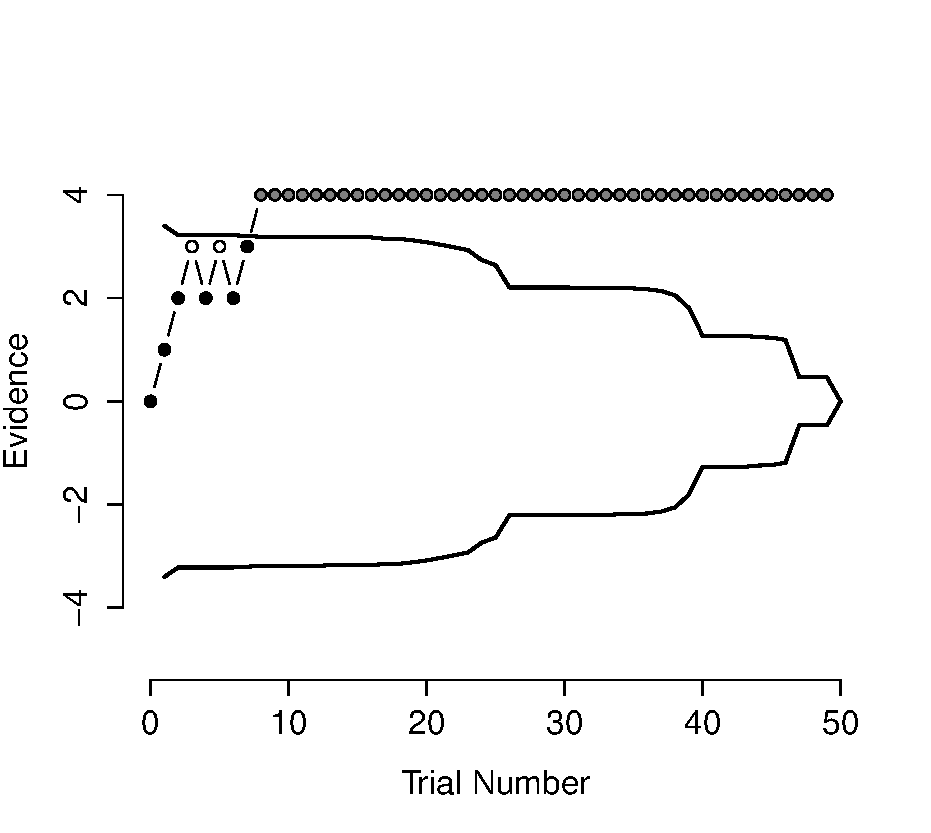
\includegraphics[scale=0.5]{./behaviourStatic.pdf} \hspace*{-.5cm}&
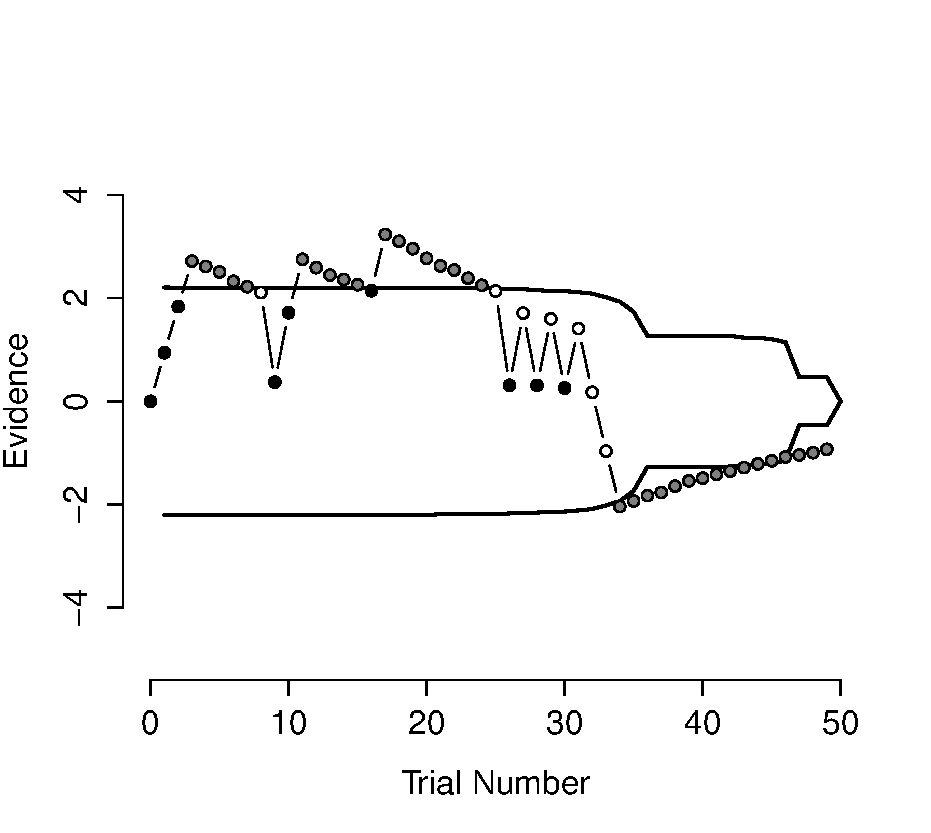
\includegraphics[scale=0.5]{./behaviourDynamic.pdf} \\
(a) & (b)
\end{tabular}
\caption{Optimal decision policies for a static 50-trial observe or bet task (panel a) and a dynamic one with a change rate of 5\% (panel b). The trial number is plotted on the x-axis, and the amount of evidence (number of As minus number of Bs) on the y-axis. The solid lines plot the decision thresholds, i.e. the amount of evidence required to justify betting. The dotted lines show the actual behavior of an agent following the policy. In a static task (panel a) the optimal decision policy leads to a pattern in which the learner observes until the evidence threshold is reached, and then bets thereafter. Black and white dots denote trials where the learner observed outcome A or B respectively, and grey dots corresponds to trials where the agent bets. When the learner believes the world can change (panel b), the evidence value actually corresponds to the estimated difference between the number of As and Bs since the last change, and it decreases over time unless observations are made. As a consequence the agent continues to make occasional observations later in the task.}
\label{fig:behavior}
\end{center}
\end{figure}

\subsectionX{What is the optimal strategy?}

As it turns out, the optimal decision strategies for the static and dynamic versions of the observe or bet task are fairly straightforward to characterize. Although the belief state $\bm{b}_t$ describes a complete distribution over $\theta_t$, for the purposes of working out what action to undertake the learner does not really need all that information: in the static task, it turns out that the optimal action is almost perfectly described in terms of $n_a - n_b$, the difference between the number of As and the number of Bs that the learner has observed so far. If this magnitude difference score exceeds a certain ``evidence threshold'', then the optimal action is to bet on whichever outcome has been more frequently observed. If the difference does not reach the threshold, then another observation should be made. The implications of this decision strategy are spelled out in Figure~\ref{fig:behavior}a, which plots the thresholds for a 50 trial observe or bet problem as a function of the trial number. At the start of the task, the optimal threshold implies that the learner needs to have observed 4 more As than Bs (or vice versa) to justify making a bet. However, the threshold value declines over time. On the final trial of the task it is never better to observe than to bet, as there is little point in collecting new information when the experiment is about to end.\footnote{The ``bumpy'' look to these curves is a somewhat uninteresting consequence of the fact that (a) evidence is discretized in this task, since each observation provides a single bit of information, and (b) the full MDP analysis makes a subtle distinction between the evidentiary value of 3 As and 0 Bs, versus 13 As and 10 Bs, and so when the complete (high dimensional) decision policy is plotted in this simple fashion, a little information is lost. There are some cases when the difference on trial 23 is exactly 3 and the model bets, and others when it observes. There are particular points in the task where this variation is amplified: essentially, when it is unclear whether a threshold of 2 is better than a threshold of 3, this subtle effect gets amplified. Thus, instead of seeing a discrete drop in the threshold from 3 to 2, we obtain this smooth transition where some belief states make the jump down from 3 to 2 before others. Note that none of this subtlety is relevant to our experiments, and we mention it only because some readers may be puzzled by the bumpy shape of the curves. The important characteristic of the thresholds is that they start high and then collapse towards zero.}

In practice, the behavior of an optimal agent in the static task agrees with the description given by \citet{tversky_information_1966}: the agent makes observations on every trial until the difference between the two outcomes exceeds a threshold, and then bets on the more frequently observed outcome for all subsequent actions. This behavior is illustrated by the dashed line in Figure~\ref{fig:behavior}a: each black dot denotes a trial on which the learner observed outcome A and each white denotes a trial on which outcome B was observed. Grey dots depict trials on which the learner chose to bet. At the start of the task, the agent makes a sequence of observations, and as a consequence the amount of evidence accrued jumps up and down as a function of the outcomes that the learner experiences. Eventually, the observed evidence level jumps above the threshold (solid black line) and the agent starts to bet. If the learner believes that the world is truly static, then placing a bet introduces no change in the learner's belief state, so the evidence accrued remains flat and the learner continues to bet for the rest of the task.

The optimal decision strategy for a learner who believes the world can change is similar in some respects, but strikingly different in others. Firstly, when the world can change the evidence is not characterized in terms of the total number of As and Bs observed since the start of the experiment. Rather, the critical quantity is the number of As and Bs observed since the last time the world changed. However, since the learner does not know precisely when the world changed, the actual quantity of interest is the learner's {\it best guess} as to how many As and Bs have been observed since the last change. More formally, the relevant quantity is the expected number of As and Bs observed since the unknown change point: the Appendix discusses how we compute this. The important consequence of this difference is that the evidentiary value of older observations declines over time: old data should only be included in the evidence tallies if the world has not changed since those observations were made. This is illustrated in Figure~\ref{fig:behavior}b. As before, the model begins by making a series of observations until a critical threshold is reached and then it starts betting, always placing bets on whichever outcome it believes to have been the more frequent one. However, because it receives no feedback during the betting phase the evidence total decreases, pushing the model's ``confidence'' back below the threshold. At that point the model starts to make observations again until the confidence gets pushed back above threshold. As Figure~\ref{fig:behavior}b illustrates, this means that the model starts the task by making a long run of observations, but then it tends to switch into a phase of alternating between runs of bets and runs of observations, always seeking to keep its confidence above the required level. Finally, there is a tendency for the task to end with a long run of bets, caused by the fact that the thresholds themselves start to collapse back towards zero right at the end of the task.

One additional difference between the static model and the dynamic model is worth highlighting: the evidence thresholds shown in the two panels of Figure~\ref{fig:behavior} are not identical. The thresholds in the dynamic world are lower than in the static one. This difference occurs for a theoretically important reason. In a static environment, it is perfectly sensible to require a lot of evidence to justify your decision making: the rewards will still be there when you switch from information collection to reward taking, so it does not hurt to be patient. In a dynamic world, you need to ``strike while the iron is hot'' because the world can change on you. A learner who patiently collects lots of evidence in a dynamic world can easily lose out because the world changes before he or she has the opportunity to take the rewards. This effect is illustrated in Figure~\ref{fig:behavior}. In the initial phase of observations, the dynamic model begins to bet after only seeing three observations. The static model sees the same three observations, but does not start betting because it requires more evidence to justify betting. As it turns out, the static model waits until eight observations have been made before it begins to bet.


\subsectionX{Deriving experimental predictions using the optimal policy}

Finding the optimal policy even for a simple task like the 50 trial observe or bet task is computationally expensive, and it seems highly unlikely that human participants are able to do so. However, this does not preclude the possibility that people are able to reason about the task sufficiently well to be able to devise a strategy that approximates it fairly well. Given this, it is useful to give careful consideration to the qualitative differences between what the model predicts people should do in the static task, and what it predicts they should do in the dynamic task. If people really are sensitive to the possibility that the world might change, then at a minimum we should expect people's strategies to shift in a manner that qualitatively agrees with the shifts made by an ideal observer when the reward structure is dynamic.

\begin{figure}[t]
\begin{center}
\begin{tabular}{cc}
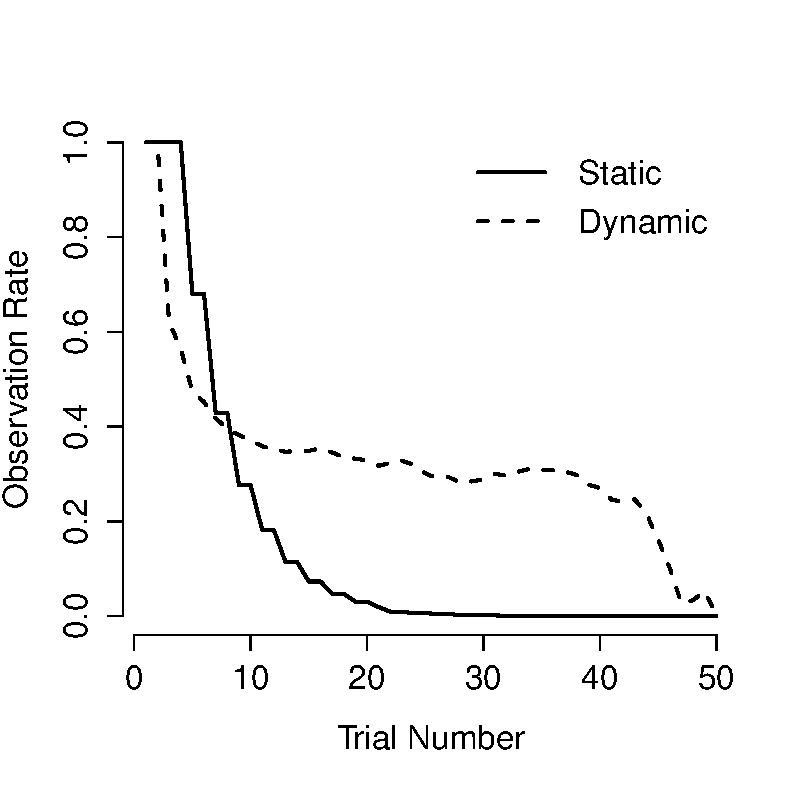
\includegraphics[scale=0.5]{behaviourOverall.pdf} &
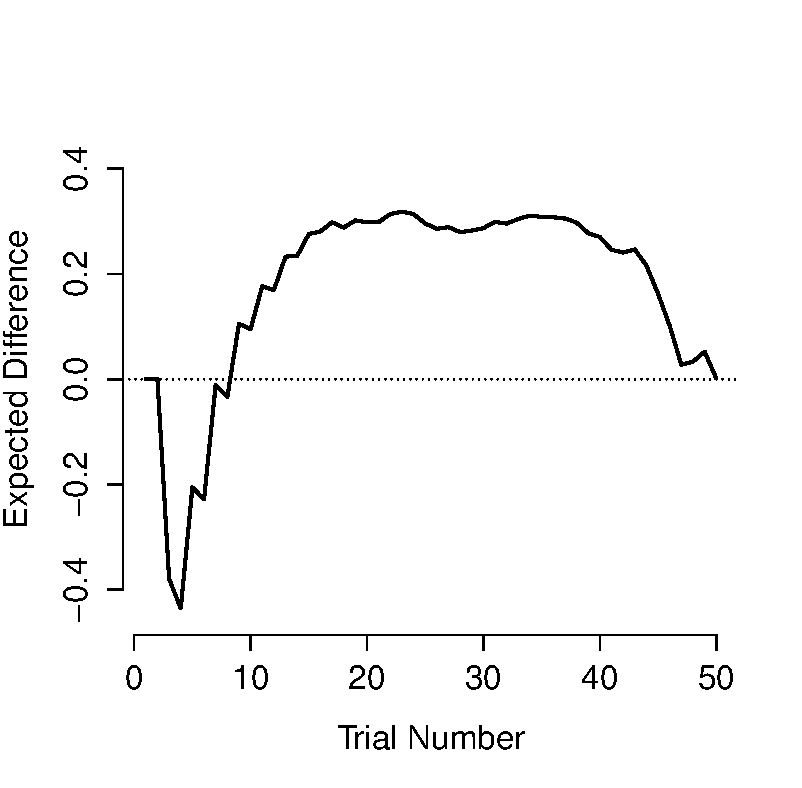
\includegraphics[scale=0.5]{behaviourDifferences.pdf} \\
(a) & (b)
\end{tabular}
\caption{Panel a: Results of simulating the optimal decision policy in a static world (solid lines) and a dynamic world (dashed lines). Each plot was constructed from 5000 simulated experiments, and shows the proportion of trials on which the agent makes an observation, broken down by trial number.  For the static world, the true change rate was always fixed at 0\%. For the dynamic world, the change rate varied randomly between 2\% and 18\%. Panel b plots the difference between the two curves, highlighting the qualitatively important prediction: observation rates in the dynamic world should be substantially higher late in the task, but slightly lower early on.}
\label{fig:qualitativeprediction}
\end{center}
\end{figure}

With that in mind, we ran simulations using the two versions of the model. For the static model, we generated 5000 random outcome sequences, each consisting of 50 trials, in which the true value of $\theta$ (i.e., the probability that the outcome will be A) was 0.75 and applied the MDP model to that sequence. For the dynamic model the simulation was similar, except that for each sequence we also selected a random change rate parameter $\alpha$ (between 2\% and 18\%) for the model and for the data sequence.\footnote{Note that these simulations are something of an approximation. In both cases the MDP model is assumed to know whether the environment is static or dynamic, and does not need to learn the rate of change. In real life this seems implausible, since people would have to infer this from their observations. However, our goal with these simplified simulations is to generate qualitative predictions that we will use to motivate experimental work, and from this perspective this simplification seems reasonable.} These simulations allowed us to count how often the model chose to make an observation, broken down by trial number. The results are shown in Figure~\ref{fig:qualitativeprediction}a. In a static environment (solid line), the observation rate drops sharply over the first few trials, and then continues to gradually decline towards zero throughout the task. In the dynamic version of the simulation (dashed line) the initial decline is even sharper: as suggested above, the optimal policy in the dynamic task genuinely does favor an earlier shift from observation to betting. However, because the dynamic task also motivates the decision maker to shift back and forth between observation and betting, the overall observation rates plateau through the middle phase of the task. It is only over the last few trials that the model shifts to a pure betting strategy, because the approaching deadline removes much of the motivation for continued information search.

An important point to recognize is that, while the simulations rely on specific parameter choices, the qualitative characteristics of the curves in Figure~\ref{fig:qualitativeprediction}a are more or less invariant: they emerge as a natural consequence of the solution to the decision problem as illustrated in Figure~\ref{fig:behavior}. Given this, while we might not expect human performance to precisely match the observation curves in Figure~\ref{fig:qualitativeprediction}a, we should expect that differences between the two versions of the task to be robust. Specifically, if we plot the differences between the two curves, as shown in Figure~\ref{fig:qualitativeprediction}b, we obtain a very striking empirical prediction about how human performance should differ in the two versions of the task: for the first few trials of the experiment, there should be a widening gap between the two conditions in which people actually observe more in the static task than the dynamic task. This difference should then rapidly reverse, and for most of the task there should be more observation in the dynamic condition. Finally, the difference tails away towards the end of the experiment. The difference curve in Figure~\ref{fig:qualitativeprediction}b represents a much stronger prediction than the obvious intuition that ``people should explore more in a dynamic environment''. Each aspect of this prediction ties to fundamental characteristics of the MDP analysis: the initial part of the curve reflects the need to strike while the iron is hot in a changing world, the middle part reflects the need to constantly monitor a changing world, and the tailing away at the end reflects the fact that the oncoming deadline removes the value of exploratory action in both environments. Given the quite unusual shape of the curve in Figure~\ref{fig:qualitativeprediction}b and its tight links to the underlying rational analysis of the task, this represents a strong prediction. In the next section, we present an experiment designed to test this prediction.




\sectionX{Experiment 1}

\subsectionX{Method}

\subsubsectionX{Participants} Data from 614 USA-based participants recruited via Amazon Mechanical Turk are reported: 56 participants were excluded for not making a single observation at any point in the experiment. A total of 246 participants self-identified as female, 363 as male, and 4 selected other/undisclosed. The average reported age was 33.2 years (sd = 15.8). The experiment took approximately 10 minutes, and all participants were paid \$US0.60 regardless of their performance.

\subsubsectionX{Procedure} The experiment was delivered online via a dedicated website. At the start of the experiment, participants were told they were taking part in a guessing game that involved ``blox machines''. The image of a blox machine showed two lights, one red and one blue. The instructions explained that on each trial of the experiment one of the two lights would turn on, but they would not necessarily be shown which light turned on. Each blox machine has a bias, explained using the following text:
\begin{quote}
{\it The lights turn on and off in an irregular way, but with a bias. Some blox machines are biased to turn on the blue light more often, and others are biased to turn the red light more often.}
\end{quote}
Participants were randomly assigned either to a {\it static condition} or a {\it dynamic condition}. In the dynamic condition, it was explained that the bias for any given machine is not fixed:
\begin{quote}
{\it A blox that used to be biased towards red can sometimes change its bias to blue, and vice versa. This doesn't happen all the time, but you should expect to see it happen a few times during this task.}
\end{quote}
No additional details were given to participants about how strong the bias is, nor were participants in the dynamic condition given any other information about how often changes might occur.

The instructions then explained that on each trial they could choose one of three actions: ``guess blue'', ``guess red'', or ``observe'', each corresponding to distinct buttons on the screen.\footnote{The ``two lights, three buttons'' set up closely mirrors the physical device used by \citet{tversky_information_1966}.} If they observed, they would be shown which one of the two lights turned on, but would forgo any opportunity to receive any points. If they guessed, the experiment would indicate that their guess had been recorded, but did not give any indication as to whether the guess was correct. The instructions explained that each correct guess would earn 1 point, and each incorrect guess would lose 1 point, and that the object of the game was to maximize the number of points gained across a total of 50 trials (the trial number was shown on screen). They were told that they would play a series of 5 such games, each with a different blox machine. To capture the ``delayed feedback'' idea, participants received feedback about their performance between games. The feedback given was quite detailed: at the end of each game participants were shown a graphical representation showing exactly which action they took on all 50 trials, as well as what the blox machine did on each trial. It showed which trials they won points for and which they lost points for, as well as giving them a final score. At the end of the experiment participants were given a completion code to claim payment via Amazon.



\begin{table}[t]
\caption{Example sequences used in the experiment. This particular pair of sequences corresponds to Game 2, Version 1. The two sequences are identical up to the change point (marked with the vertical line), which occurs on trial 17 in this instance. Prior to the change point, Option A (black dots) occurs more frequently. After the change point, in the static condition this trend continues, with black remaining the more common outcome. In the dynamic condition, all outcomes after the change point are reversed, so Option B (white dots) is the better choice after trial 17. Participants were not told the specific nature of these changes.}
\label{tab:seq}
\begin{center}
\begin{tabular}{ll}
\footnotesize Static: &\footnotesize $
 \bullet \! \bullet \! \bullet \! \bullet \! \circ \! \bullet \! \circ \! \bullet \! \circ \! \circ \! \bullet \! \bullet \! \bullet \! \bullet \! \bullet \! \bullet  | \bullet \! \bullet \! \circ \! \bullet \! \bullet \! \circ \! \bullet \! \bullet \! \bullet \! \bullet \! \bullet \! \circ \! \bullet \! \bullet \! \bullet \! \bullet \! \bullet \! \circ \! \circ \! \bullet \! \bullet \! \bullet \! \bullet \! \bullet \! \bullet \! \circ \! \bullet \! \bullet \! \bullet \! \bullet \! \circ \! \circ \! \circ \! \bullet
 $ \\
\footnotesize Dynamic: &\footnotesize $
 \bullet \! \bullet \! \bullet \! \bullet \! \circ \! \bullet \! \circ \! \bullet \! \circ \! \circ \! \bullet \! \bullet \! \bullet \! \bullet \! \bullet \! \bullet  | \circ \! \circ \! \bullet \! \circ \! \circ \! \bullet \! \circ \! \circ \! \circ \! \circ \! \circ \! \bullet \! \circ \! \circ \! \circ \! \circ \! \circ \! \bullet \! \bullet \! \circ \! \circ \! \circ \! \circ \! \circ \! \circ \! \bullet \! \circ \! \circ \! \circ \! \circ \! \bullet \! \bullet \! \bullet \! \circ \!
 $ \\
\end{tabular}
\end{center}
\end{table}



\subsubsectionX{Materials}

The sequence of outcomes produced by the blox machine was fixed ahead of time. There were 2 between-subject conditions (static and dynamic), 3 between subject ``versions'' (discussed below) and 5 within-subject games, yielding a total of 30 distinct outcomes sequences listed in the Appendix. For the static condition the sequences were generated pseudo-randomly. Across the 15 sequences the average proportion of high frequency outcomes was 78\%. Red was the high frequency outcome for 7 of the sequences, and blue for the other 8.

The stimulus sequences in the dynamic condition were constructed from the static sequences via the following procedure. A ``change point'' was selected (constrained to lie between trial 15 and trial 35): all outcomes prior to the change point were exactly identical to their counterpart in the static sequence, and all outcomes after the change point were reversed. An example of a sequence produced in this fashion is shown in Table~\ref{tab:seq}. For all three versions of the dynamic task, 4 of the 5 sequences were altered in this fashion, and one was left unchanged: given 4 changes across 250 trials, the empirical change rate in the task was 1.6\%. Across the 12 altered sequences, the average rate of the high frequency outcome prior to the change points was 75\%. After the change points, the rate of the now low frequency outcome fell to 21\%.

The location of the change point in every game is listed in Table~\ref{tab:changepoints}. As the table makes clear, participants in Version 1 of the dynamic condition did not see any changes during Game 1, whereas in Version 2 it was Game 3 that did not contain a change point, and in Version 3 it was Game 5. In these cases the stimulus sequence was identical in the static and dynamic versions of the task, allowing us to examine the ``pure'' effect of expectations about change independent of any effects of the stimulus sequence itself.


\begin{table}[t]
\caption{Trial number upon which the change occurred, in all three versions of the dynamic condition. Note that in all three versions there is one game in which no change actually occurred. In these cases the sequence of outcomes in the dynamic condition was identical to the sequence used in the static condition.}
\label{tab:changepoints}
\footnotesize
\begin{center}
\begin{tabular}{l|rrrrr}
& Game 1 & Game 2 & Game 3 & Game 4 & Game 5 \\ \hline
Version 1 & None & 17 & 26 & 29 & 22 \\
Version 2 & 35 & 16 & None & 20 & 18 \\
Version 3 & 23 & 17 & 19 & 20 & None
\end{tabular}
\end{center}
\end{table}


Throughout the results, we refer to Option A as the high frequency outcome in a static sequence, regardless of whether that corresponds to the red or blue light. In the dynamic condition Option A refers to the option that is initially high frequency, but later (in 4 of 5 cases) becomes low frequency.

\subsectionX{Results}


\subsubsectionX{Observation behavior at the aggregate level}

The proportion of participants making observations on each trial of the experiment is shown in Figure~\ref{fig:obsByGame}, broken down by condition and game number and averaged across the three different versions. The results follow the same basic profile predicted on the basis of the optimal model shown in Figure~\ref{fig:qualitativeprediction}a. In both conditions, people almost always observe on the first trial (88\% for the static condition, 84\% for the dynamic condition). In the static condition the observation rate consistently declines throughout the task, and by the final trial the rate of observation has fallen to 3\%. In the dynamic condition, however, the observation rate stabilizes throughout the middle portion of the task. From trials 15 to 35, the average observation rate was 23\%, and displayed almost no variation over that time frame: the highest observation rate over that range was only 27\% (on trial 21) and the lowest was 20\% (trial 35). However, with the end of task acting as a deadline that limits the value of new observations even in the dynamic condition, the observation rate declined over the last few trials of the experiment, with observation rates on the final trial being 12\%.

\begin{figure}[p]
\begin{center}
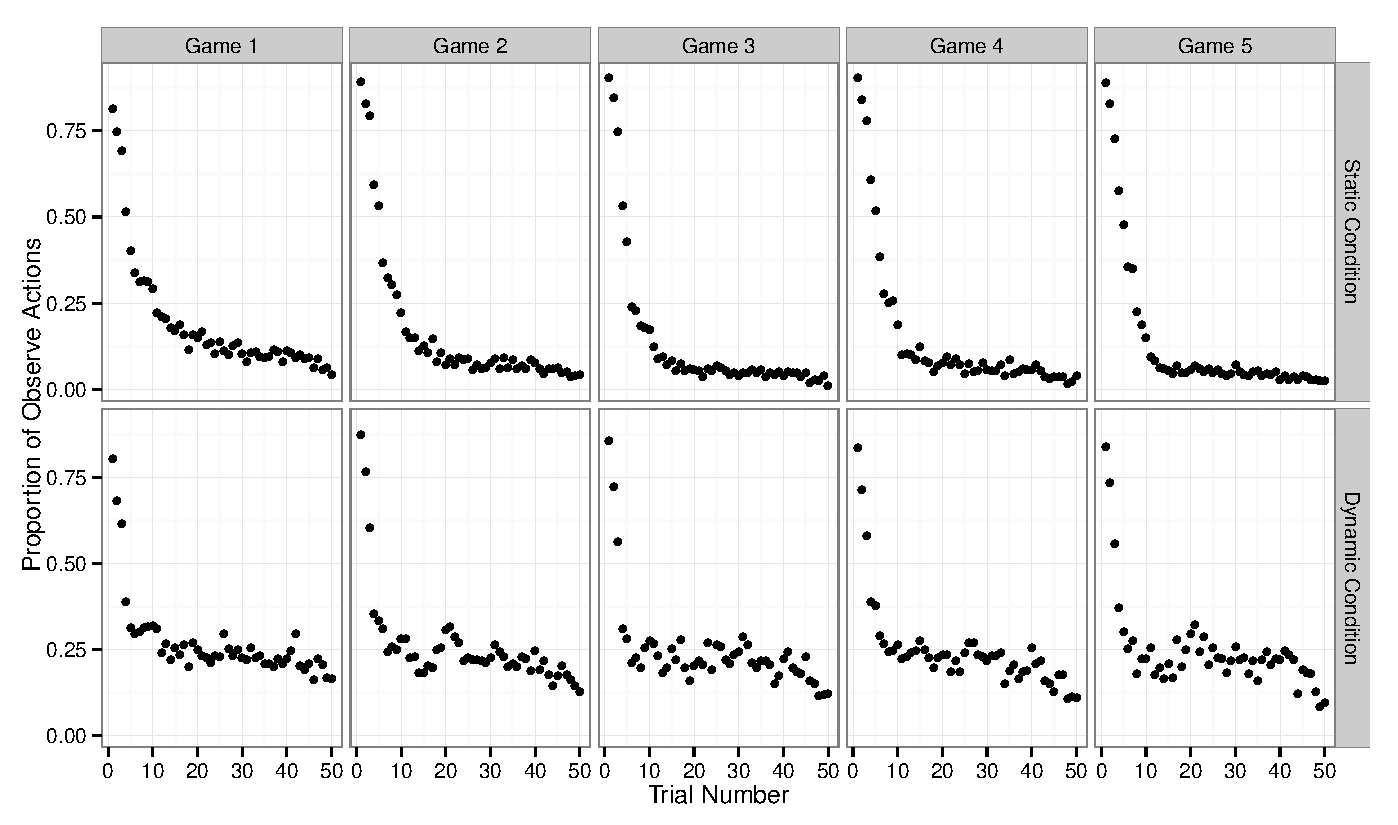
\includegraphics[scale=.6]{obsByGame.pdf}
\caption{Average proportion of observe actions, broken down by trial number, game number and condition. In all cases, participants observe with high probability during the first few trials. Consistent with the qualitative predictions made by the rational analysis, in the static condition the observation rate continues to decline to near zero, whereas in the dynamic condition it tends to plateau at a constant level until near the very end of the task.}
\label{fig:obsByGame}
\end{center}
\end{figure}

\begin{figure}[p]
\begin{center}
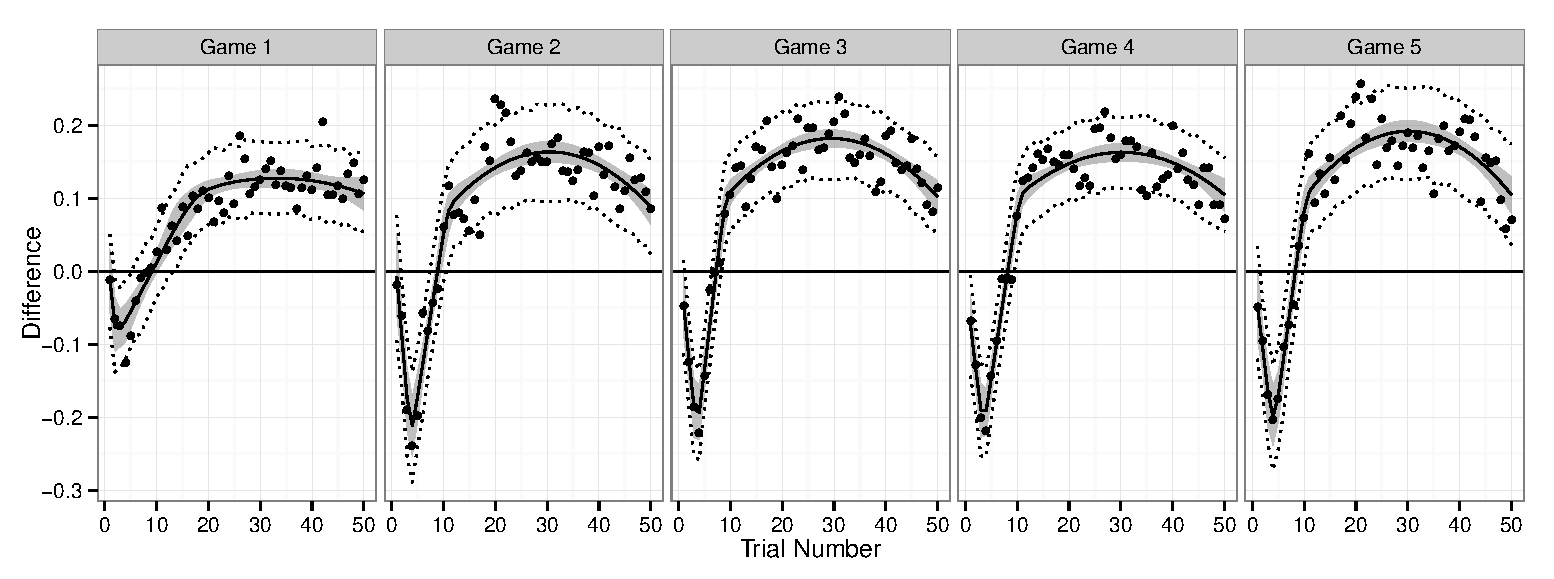
\includegraphics[scale=.6]{diffByGame.pdf}
\caption{The difference in observation probabilities between conditions, plotted separately for each game. Shaded area denotes the Bayesian 95\% credible interval for the mean. Dotted lines show the 5th and 95th quantiles of the posterior predictive distribution.}
\label{fig:diffByGame}
\end{center}
\end{figure}



As noted in the introduction, the MDP analysis of the observe or bet task makes quite strong predictions about the differences between the two conditions. It does not merely predict higher observations rates in the dynamic condition. Rather, if the demands of different environments are genuinely placing a strong constraint on people's decision making strategies in the task, then the difference between the observation rates across conditions should have the same qualitative character as the curve shown in Figure~\ref{fig:qualitativeprediction}b. We formalize the prediction in Figure~\ref{fig:qualitativeprediction}b using a three segment Bayesian regression model implemented in JAGS \citep{plummer_jags:_2003}: the first and second segments are linear, while the third is quadratic. The edges of the different segments are treated as latent variables, as are the regression coefficients themselves. The formal specification of the data analysis model is given in the Appendix.

Applying this model to the difference data shows a high degree of agreement. The model fits are shown in Figure~\ref{fig:diffByGame}. The solid line shows the estimate of the regression function, the shaded regions depict Bayesian 95\% credible intervals for the difference at each trial, and the dotted lines show 95\% credible intervals for the raw data. The difference between conditions very closely agrees with the qualitative prediction made by the MDP analysis, especially for Games 2-5.

\subsubsectionX{The effect of expectations about change}

For the most part, the differences in Figure~\ref{fig:obsByGame} reflect both the participant strategy choices and the interaction between those strategies and the environment. A more direct measure of how people's expectations influence behavior can be obtained by looking at those cases where the static and dynamic conditions used identical sequences: Game 1 of Version 1, Game 3 of Version 2 and Game 5 of Version 3. The observation profiles for these cases are plotted in Figure~\ref{fig:obsSpecial}, and the differences between conditions and corresponding regression analyses are plotted in Figure~\ref{fig:diffSpecial}. As is clear from inspection of these plots, the effect that we observe on Games 3 and 5 is essentially unchanged from the corresponding plots in Figures~\ref{fig:obsByGame} and~\ref{fig:diffByGame}. Once people have some familiarity with the task the different observation profiles are heavily driven by their {\it beliefs} about the changeability of the environment.

Looking at the profiles for Game 1 in Figures~\ref{fig:obsSpecial} and~\ref{fig:diffSpecial} reveals a subtly different story. In this case participants have no prior experience with the task, no knowledge about when the changes might occur or what form they might take (in the dynamic condition), and as it turns out the actual sequence of observations contained no changes at all regardless of condition. The only difference in this instance is the cover story. The results show a greatly attenuated version of the effect: in the dynamic condition people do make more ``late'' observations, but there is no equivalent tendency to make more observations in the static condition early in the task. That being said, it is difficult to know how to interpret this pattern: although we included this case in order to have a direct analog of the dynamic condition from \cite{tversky_information_1966}, it is a somewhat odd condition to consider at all, because it is somewhat deceptive. In the dynamic condition participants were told to expect changes, yet in the very first task they undertook there were none to be found.



\begin{figure}[p]
\begin{center}
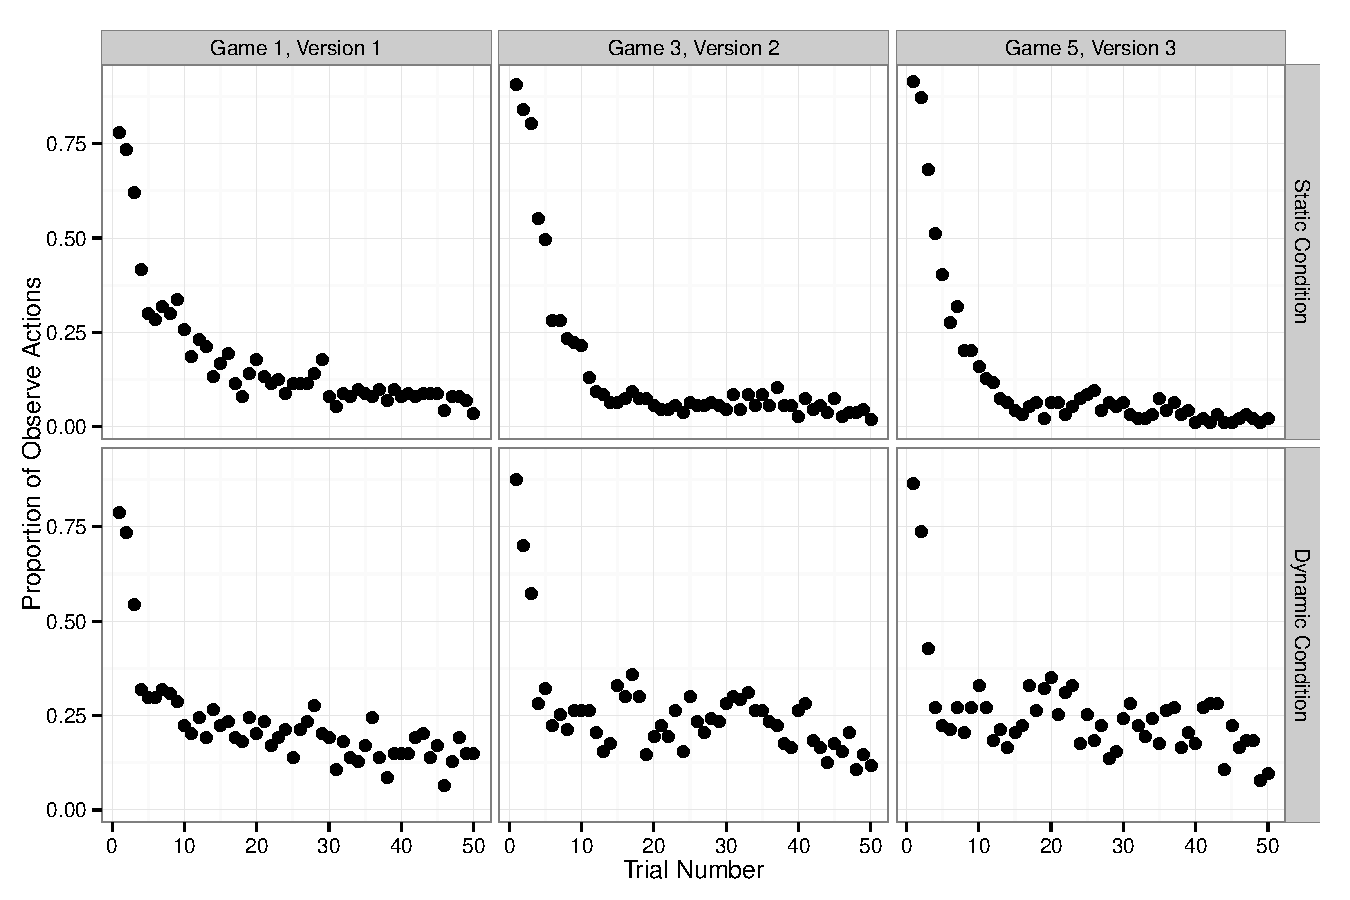
\includegraphics[scale=.5]{dataSpecialCases.pdf}
\caption{The effect of expectations about change. Human observation rates in those instances when no changes occurred in the dynamic condition, and thus the stimulus sequence was identical in both the static and dynamic conditions. The pattern of results is consistent with the overall pattern in Figure~\protect\ref{fig:obsByGame}, illustrating that people's expectation that changes can occur are sufficient to drive a difference in performance.}
\label{fig:obsSpecial}
\end{center}
\end{figure}


\begin{figure}[p]
\begin{center}
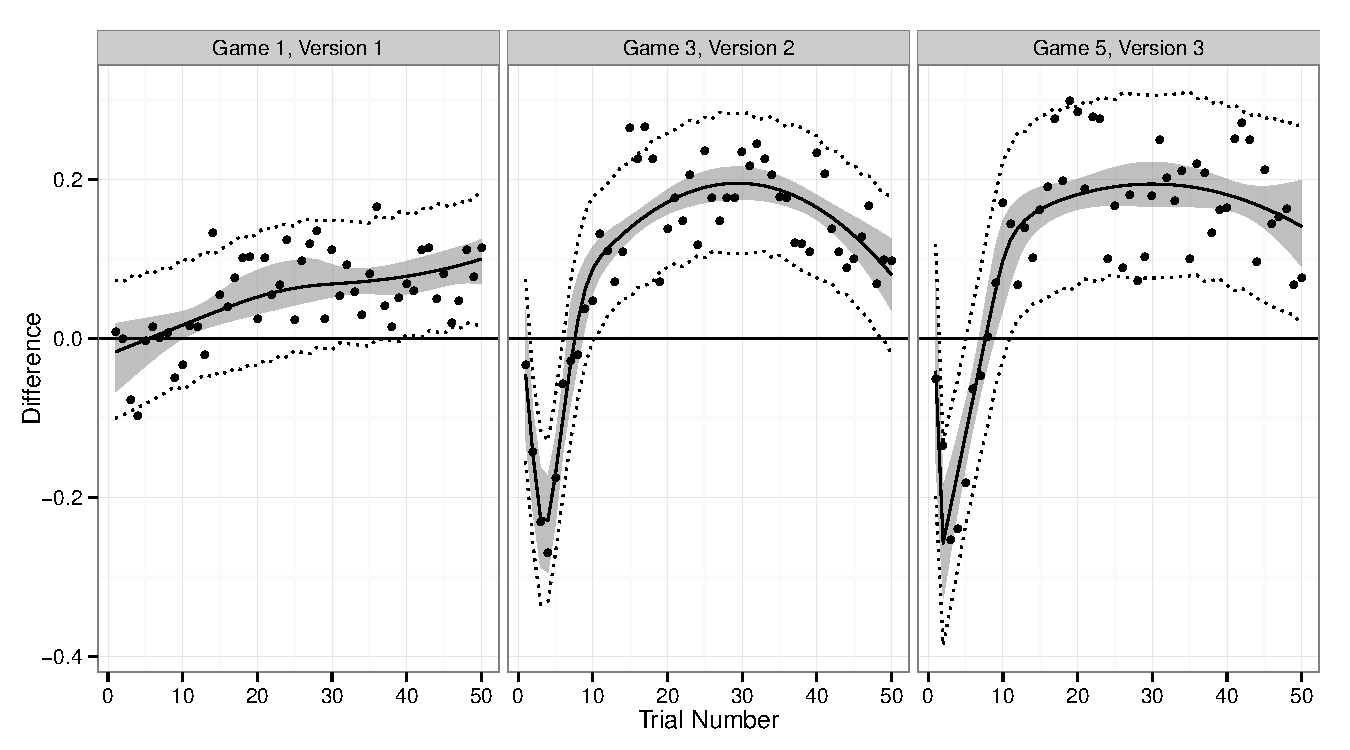
\includegraphics[scale=.5]{allDiffs.pdf}
\caption{The difference in observation probabilities between conditions, plotted only for the special cases where the underlying sequences were identical in the static and dynamic conditions. Shaded area denotes the Bayesian 95\% credible interval for the mean. Dotted lines show the 5th and 95th quantiles of the posterior predictive distribution.}
\label{fig:diffSpecial}
\end{center}
\end{figure}


\subsubsectionX{Observation strategies at the individual subject level}


A second way to examine model predictions is to consider the behavioral patterns produced by the MDP analysis at an individual subjects level when the task is assumed to be static (i.e., Figure~\ref{fig:behavior}a) versus when it is assumed to be dynamic (i.e., Figure~\ref{fig:behavior}b). In the static environment, the optimal strategy for any given instance of the observe or bet task is to have all observations precede all bets. We refer to this as the strict ``front loading'' strategy, in which all observations come first. The smooth curves shown at the aggregate level arise primarily because of variability in the specific sequence of outcomes. In the dynamic environment, this pattern does not hold. Instead, it is expected that observations be distributed throughout the task even at the individual subject level.

To what extent is this prediction satisfied by human participants? Figure~\ref{fig:frontload2} plots the proportion of subjects who follow the strict front loading strategy, broken down by condition and game number. When the environment is dynamic, almost no-one uses this strategy: the proportion of front loading ranges from 5\% to 10\%, with no discernible pattern across games. The static conditions show a marked contrast: even on Game 1, the proportion of subjects who strictly front load the observations is 24\%. As participants become familiar with the task, this proportion rises rapidly, so that by Game 5 fully 62\% of participants are behaving exactly in accordance with the strict front loading strategy.

\begin{figure}[t]
\begin{center}
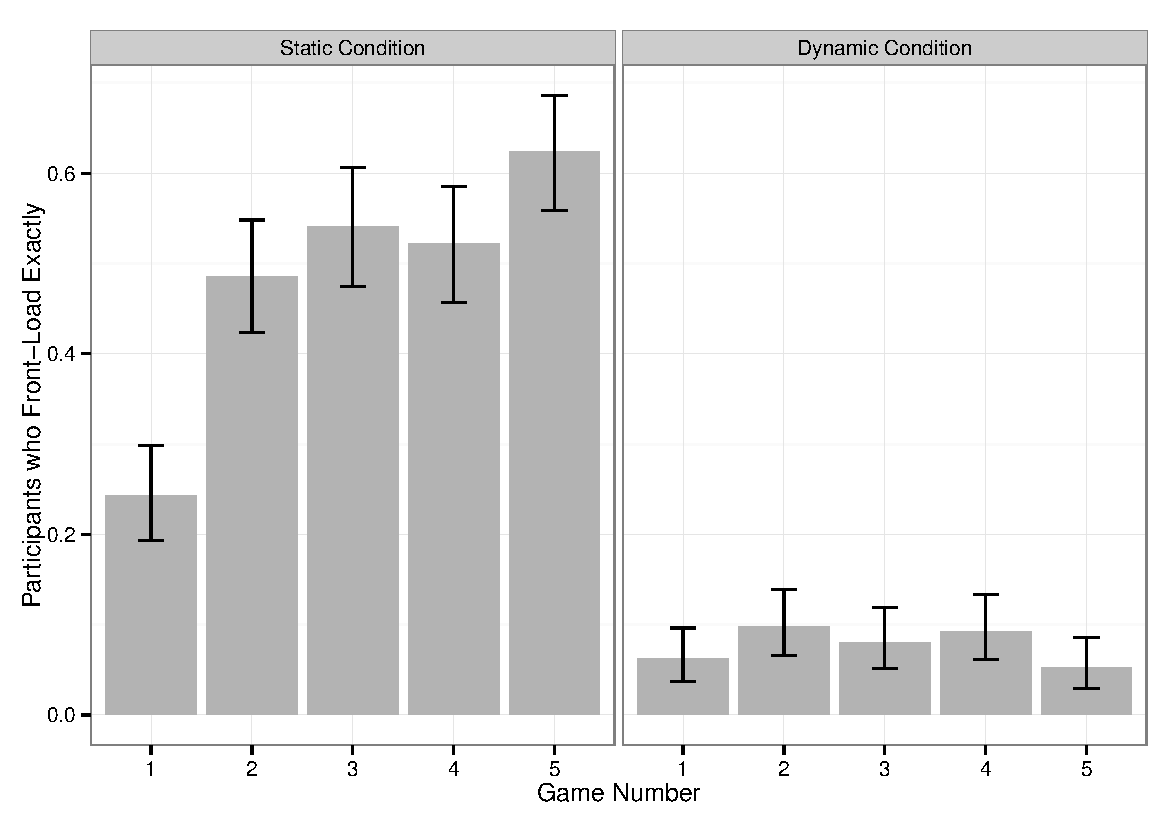
\includegraphics[scale=.5]{frontLoading2.pdf}
\caption{Proportion of participants who front load all of their observations, plotted separately by condition and game number. Error bars show 95\% Bayesian credible intervals for an unknown proportion under a Jeffreys prior.  }
\label{fig:frontload2}
\end{center}
\end{figure}




The analysis depicted in Figure~\ref{fig:frontload2} adopts a very strict definition of the front loading strategy. An alternative view is to characterize the observation behavior in terms of the proportion of observations that occur during the first half of the task. Under a front loading strategy, this quantity is expected to be fairly close to 100\%. This weaker criterion is almost always satisfied in the static condition: the median value for the first observe or bet game is 87.5\%, and is 100\% for all subsequent games. Compare this to the corresponding numbers for the dynamic condition, in which participants spread their observations throughout the task. The median proportion of first half observation did not change much across games, ranging from 57\% to 60\%, and (apart from a small group of subjects who front loaded all their observations) did not vary greatly among individuals. In almost all cases, people made almost as many observations in the second half of the task as they did in the first half.



\subsubsectionX{Betting strategies}

\begin{figure}[t]
\begin{center}
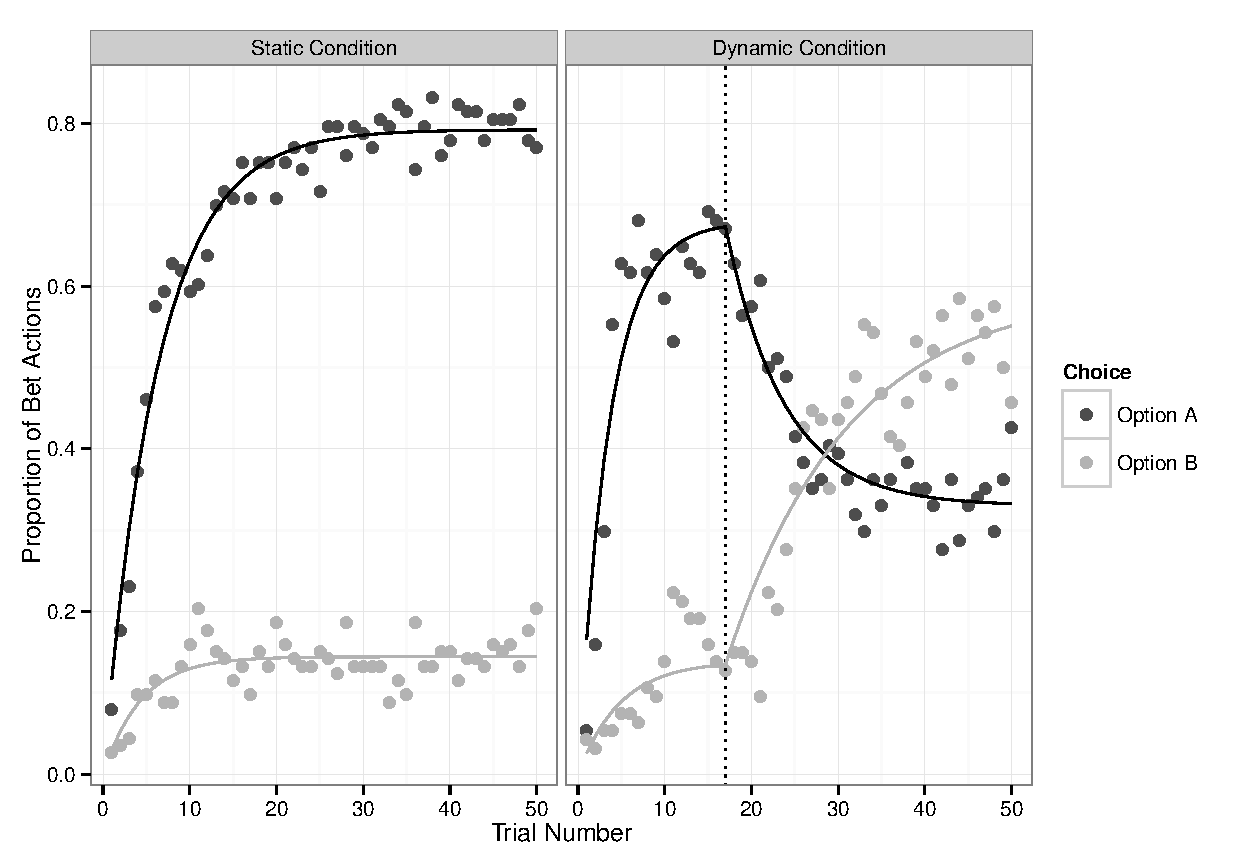
\includegraphics[scale=.5]{bettingExample.pdf}
\caption{Proportion of people betting on the different options for a specific stimulus sequence (Game 2, Version 1: see Table~\ref{tab:seq}). In both plots, ``Option A'' refers to the more-probable outcome on trial 1. For the dynamic condition, Option A is the better option for the first 17 trials, and Option B is better for the rest of the task. The pattern of bets shown here is grossly typical of all games and sequences.}
\label{fig:bettingExample}
\end{center}
\end{figure}

Up to this point we have focused the discussion on how people choose to allocate their observations, because this is where the MDP analysis makes critical predictions. Nevertheless, it is also instructive to consider the strategies that people use to make bets. To give an illustrative example, Figure~\ref{fig:bettingExample} plots the proportion of subjects choosing to bet, plotted across all 50 trials for one specific outcome sequence (Game 2, Version 1). In the static condition, the proportion of subjects betting on the better option (Option A) starts at zero and then rises rapidly, levelling out at about 80\% of all actions. A similar pattern is seen for Option B, but it levels out at about 15\% of actions taken. The remaining 5\% of actions are observations. In the dynamic condition, a similar pattern is observed at the beginning, but after the change occurs on trial 17, the betting proportions shift, and people begin to allocate more bets to Option B. Although this figure only plots the data from a single outcome sequence, it is a very typical one.\footnote{To draw the curves plotted in Figure~\ref{fig:bettingExample} we estimated a simple exponential rise to asymptote function for the static condition. The formula for the curve is $y(t)=a(1 - e^{-bt})$ where $a$ is the asymptote and $b$ is the rate of change. For the dynamic condition we estimated a two-stage model. Prior to the change point $c$, we again use the function $y(t)=a_1(1 - e^{-b_1t})$. For trials $t>c$ after the change point, the curve is an exponential shift-to-asymptote but with a new asymptote and new rate, giving $y(t) = y(c) + (a_2 - y(c))(1-e^{-b_2(t-c)})$ as the function. There is no theoretical reason for these choices, and other possibilities (e.g., logistic) exist. Moreover, unlike the observation profiles in Figures~\protect\ref{fig:diffByGame} and~\protect\ref{fig:diffSpecial} we did not have any genuinely {\it a priori} hypotheses about the form of the betting curves, and as such we felt it was inappropriate to convert our {\it post hoc} curve fitting exercise into a fully-fledged regression model. We fit these curves to the data solely for the purpose of improving the readability of the figure, not to make a substantive claim about human cognition, though we note in passing that this family of curves seems to work quite well across most games and versions.}


Examining the responses for the static condition suggests a choice pattern much in line with frequent findings from typical probability learning tasks, and other investigations of the observe or bet task: with some prior task experience (Game 2 and beyond), people over-match when allocating their bets \citep[e.g.,][]{shanks_re-examination_2002,rakow_role_2010}. If we consider only those trials on which participants placed a bet (i.e., ignore observations), Figure~\ref{fig:bettingExample} implies that by the end of the task participants were allocating about 85\% of their bets on Option A.\footnote{Note that Figure~\ref{fig:bettingExample} does not ignore observations: it plots the raw frequencies of the two bet options, and so the heights of the two curves do not sum to 1.} Given that the proportion of Option A outcomes in this particular sequence is only 75\%, it would appear that participants did not follow a pure probability matching strategy either \citep[see][for a review]{vulkan_economists_2000}. In other words, while participants did not strictly maximize when placing their bets, they adopted betting strategies that outperformed a simple matching heuristic. However, when we consider the dynamic condition, it is far less clear from this ``two part'' curve what we should conclude about whether participants were probability matching.

Once again, however, we can turn to the MDP analysis presented in the introduction to assist in understanding participant behavior. As illustrated in Figure~\ref{fig:behavior}, the critical characteristic of the betting strategy adopted by a purely rational agent in this task is {\it internal consistency} within a run of bets. That is, if a participant makes a sequence of bets with no observations in between them, a rational agent should place all of those bets on the same option. An optimal decision policy for this task does allow the agent to switch between options, but the MDP model predicts that this can only happen when the agent makes new observations and updates his or her beliefs accordingly. An example of this is shown in Figure~\ref{fig:behavior}b: the first three runs of bets made by the MDP model all occur because the evidence has pushed the model's ``confidence'' above the threshold, and so all bets in those runs are all on the same option. In contrast, the fourth run of bets occurs when new observations push the model to believe the other option is superior, and so all bets within that run are placed on that option. At a qualitative level, this kind of belief change is what underpins the empirical reversal shown on the right hand side of Figure~\ref{fig:bettingExample}: that is, in a dynamic world participants use their observations to guide belief changes and therefore reversals in their betting strategies. However, the MDP analysis does not merely predict that people will reverse their betting strategies when the world changes: it also makes the prediction that every run of bets should be placed on the same option.

%\begin{figure}[t]
%\begin{center}
%\includegraphics[scale=.5]{betConsistency.pdf}
%\caption{Proportion of participants who maintained perfect consistency within all betting runs, broken down by condition and by game number. Error bars show 95\% credible intervals.}
%\label{fig:betConsistency}
%\end{center}
%\end{figure}

Not surprisingly, only a minority of participants adopt betting strategies that are perfectly consistent with this strict internal consistency requirement. Strict internal consistency was satisfied only in 28\% of games in the static condition, and in 21\% of games in the dynamic condition. To get a finer grained perspective on the individual behavior, we can disaggregate the data further and look at  individual betting runs. When we do so it turns out that there is a remarkably high proportion of consistent runs. Figure~\ref{fig:overMatching} plots the number of consistent betting runs (black bars) against the total number of runs (grey bars), broken down by run length and condition. Irrespective of how long the run of bets is and what condition we consider, it is clear that the vast majority of betting runs are in fact perfectly consistent. To give a sense of just how unlikely this is, the white error bars plot the 95\% credible interval for the number of consistent runs we would expect if people adopted a probability matching strategy {\it within} betting runs. Given the massive overrepresentation of consistent betting runs at almost every run length, it seems safe to conclude that, at a bare minimum, participants betting behavior reflected some form of overmatching strategy.


\begin{figure}[t]
\begin{center}
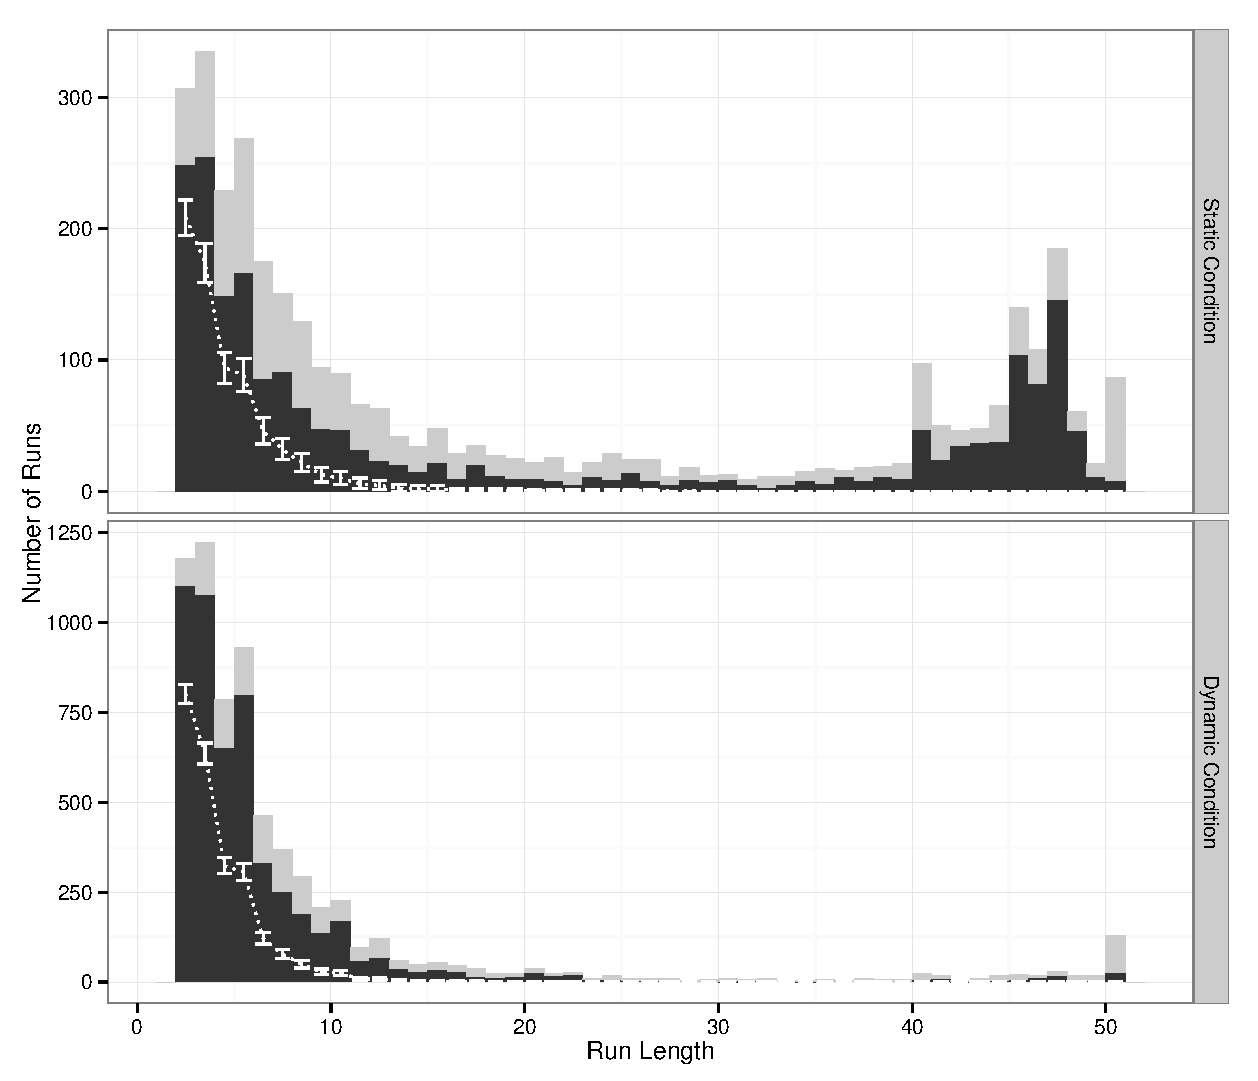
\includegraphics[scale=.6]{overMatching.pdf}
\caption{Number of consistent betting runs, broken down by run length and condition. The heights of the black bars depict the number of consistent runs, and the grey bars show the total number of runs of the corresponding run length. The white error bars show the expected 95\% intervals for the number of consistent runs if participants were probability matching (at 80\%).}
\label{fig:overMatching}
\end{center}
\end{figure}

\subsectionX{Discussion}

The manipulation produced almost exactly the predicted effect with regards to observation profiles. A surprising proportion of people follow a strict front-loading strategy for their observations in the static condition, while almost nobody does in the dynamic condition. The betting strategies are less straightforward to characterize, and only a minority of participants match the strict internal consistency criterion. Nevertheless, at the level of individual betting runs there is a remarkably high proportion of perfectly consistent betting streaks regardless of how long the run is, a pattern that is grossly inconsistent with the usual probability matching effect. Thus, while not strictly optimal in allocating bets, people were very clearly overmatching to the sequence.

A critical point to make about all of these results is that none of them make any sense if (for instance) the tendency to make occasional non-front loaded observations when given static sequences is solely due to cognitive limitations. For instance, if the reason such observations are made is due to memory limitations,\footnote{This is not to say that memory limitations have no role to play in understanding the task, and \citet{rakow_role_2010} do find that memory capacity relates to performance in the static task. However, our results also highlight that there are good strategic reasons for people to avoid strict front loading.} why should they become more common in the dynamic condition? If people were not sensitive to some notion of what counts as an optimal decision policy, why do we see the proportion of observations decline sharply in the last few trials of the task?  Perhaps most remarkably, if participants were not highly sensitive to the value of evidence in different environments, why do they observe {\it less} often in the first few trials of the dynamic condition and more often thereafter. The MDP analysis explains the asymmetry for the first few trials quite elegantly: formally, the effect is caused by the subtle lowering of the thresholds shown in Figure~\ref{fig:behavior} when the change rate is increased. But the deeper reason for why this threshold shift occurs is the ``strike while the iron is hot'' effect discussed earlier: if the world can change on you, it is a bad idea to collect too much evidence because it might change before you have the opportunity to exploit the knowledge it provides. Later on, the difference between conditions reflects the obvious ``keep your eyes peeled'' strategy: if the world can change on you, it is occasionally necessary to shift back to exploratory behavior even after the initial explore to exploit shift has occurred, because when the world changes a previously good strategy can become bad.

One particularly interesting finding with regards to observation strategies is that people did not properly front-load their observations in the first game in the static condition, as one might expect if they were adopting a near optimal strategy \citep[cf.][]{rakow_role_2010,tversky_information_1966}. On the one hand, the steep rise in front loading rates shown in Figure~\ref{fig:frontload2} suggests that people can and do learn the optimal strategy (or something very much like it) from experience, to the point that by the end of a 10 minute task almost two-thirds of participants followed a strict front loading strategy. On the other hand, this raises the question of why only about a fifth of participants were able to do so on the first attempt.

Two possibilities suggest themselves. The first possibility is distrust. If participants did not completely trust the cover story presented to them, then it would be foolish to commit to a strict front loading strategy on the first game. More formally, an agent who is uncertain about whether the world can change is obligated to act as if change is a real possibility. In the observe or bet task this means that the agent needs to make observations later in the task in order to {\it infer} whether the world can change. Given the number of psychology experiments that involve deception, and (more importantly) the number of real life scenarios when the reality does not match the textbook description, one might forgive participants for bringing a certain degree of skepticism to the task.

The second possibility is that participants require trial-by-trial experience in the task before they can fully appreciate the implications of the described problem. That is, in order to hit upon the right strategy (front loading) they need to experience the differential effect of distributing versus concentrating observation trials \citep[e.g.,][]{newell_role_2007,newell_probability_2013}. To a statistically trained reasoner who finds themselves in the static condition, it might be perfectly obvious on the basis of the simple verbal description we provided that the output of the blox machine can be characterized as a Bernoulli sequence with unknown success probability,\footnote{Obvious, but not strictly correct. A few of the sequences generated the first time were highly regular to the human eye, and we resampled them in order to avoid confusing participants: as such, the actual sequences used cannot be characterized as pure Bernoulli sequences, though admittedly the deviations are small. The larger point remains though: real life is far messier than any description of it might imply.}  and such a reasoner might indeed be able to infer that observations should precede actions in all cases when this assumption holds. However, this strikes us as a very abstract form of reasoning, and it is not at all clear that we should expect people to be able to reason optimally about a task with which they have no direct experience.

So which is it? Do people require direct experience of the observe or bet task in order to {\it construct} an approximately optimal strategy, or do they need to be convinced to trust the experimenter in order to be willing to {\it adopt} it? It is this question that motivates Experiment 2.



\sectionX{Experiment 2}

To tease the two candidate explanations apart, we created a version of the task designed to inspire as much trust as we possibly could. In Experiment 2, we ran the study in the lab, using a physical deck of playing cards to generate random outcomes instead of using a computer to generate (easily faked) outcomes. The task allowed participants to verify that the deck of cards was composed either of 70\% red cards or 70\% black cards, and to verify that the decks were properly shuffled, but did not allow them to know whether their deck was mostly red or mostly black. Given this, the participants should have no real reason to distrust the scenario, and so if distrust is the explanation, the front loading strategy should be adopted immediately. In contrast, if a lack of trial by trial experience is the explanation, participants would not be expected to front load their observations when doing the task, but they should be expected to realize at the end of the task that their strategy was incorrect.

\subsectionX{Method}

\subsubsectionX{Participants} 30 undergraduate students (16 female, 14 male) from the University of New South Wales participated in this experiment in exchange for course credit. Additionally, participants could earn a performance based monetary payoff. The average age of participants was 18.8 (sd = 1.4).


\subsubsectionX{Materials and Procedure} In order to maximize trust in the random nature of the sequence, the following procedure was used. Participants were seated at a table across from the experimenter and presented with two decks of 100 cards each, one consisting of only red cards (hearts), the other of only black cards (spades). Participants were given a chance to verify the composition of both card decks before the experimenter visibly exchanged 30 cards between the decks, so that each deck was biased towards either red or black to the same magnitude (70:30). Both decks were then thoroughly randomized using a shuffling machine and placed in transparent containers. These containers were then placed in a larger box. The experimenter shuffled this box with both containers, before the participant randomly picked one of the containers and hence the deck it contained to play with in the guessing game.

After a deck was selected, it was placed face down on a table and the card guessing game commenced. On each trial  participants could choose to either observe the top card in the deck (but receive no money) or to guess the color of that card without being shown what it was. With each choice, one card was moved forward, either face down or up, depending on whether the participant had opted to observe that particular card. Cards were not replaced back in to the deck.\footnote{The sampling without replacement scheme used in Experiment 2 differs from the sampling with replacement scheme in Experiment 1, but while that does have some implications for computing optimal strategies the differences are minor unless the agent makes a very large number of observations.} At the end of the game, participants were informed about their guessing success and payoffs. To help ensure participants were motivated, they were paid on the basis of performance in addition to receiving course credit. For each correct guess, they received AUD\$0.10; for each incorrect guess, a loss of AUD\$0.10 was incurred. Negative total scores resulted in no payoffs.\footnote{It is worth noting that the rewards offered in Experiment 2 are far more performance based than in Experiment 1, but (to foreshadow the results somewhat) there is no evidence that participants performed better. If anything, participants in Experiment 1 performed better.}

Following the card guessing game, participants were asked to complete a short questionnaire querying their knowledge of the card deck composition and their strategy use during the game. In particular, it asked them to consider four hypothetical choice strategies for the card game: (a) never observe, always guess a color; (b) observe for a few trials at the start of the game; then always guess a colour for the rest of the game; (c) going back and forth between observing and guessing throughout the entire game; and (d) never guess, always observe the card. They were asked to indicate which of these strategies best describes what they did, which one they think would have made the most money, and which one they would follow if they were given the opportunity to do the task again \citep[cf.][]{koehler_probability_2010}.

\subsectionX{Results}

The raw data for the experiment are plotted in Figure~\ref{fig:realLifeChoices}, and are consistent with the results for Game 1 of the static condition in Experiment 1, though the data are understandably noisier given the much smaller sample size. Only 5 of the 29 participants (17\%) followed the strict front loading strategy, similar to the 24\% of participants who did so in Game 1 of the static condition earlier. The median proportion of first half observations was 80.6\%, which is broadly consistent with the 87.5\% figure from the previous experiment, though the two are not perfectly comparable. Given the different number of trials (100 versus 50) and the fact that a big ``spike'' of observations is expected right at the beginning, the slightly lower proportion in Experiment 2 makes sense. Similarly, the betting proportions shown in Figure~\ref{fig:realLifeChoices} are broadly similar to those shown in the left hand panel of Figure~\ref{fig:bettingExample}. Overall, the pattern of behavior during the task itself does not show any substantial differences from the previous experiment, which provides suggestive evidence that the measures taken to increase participants' trust in the static world assumption made no difference to performance.

\begin{figure}[t]
\begin{center}
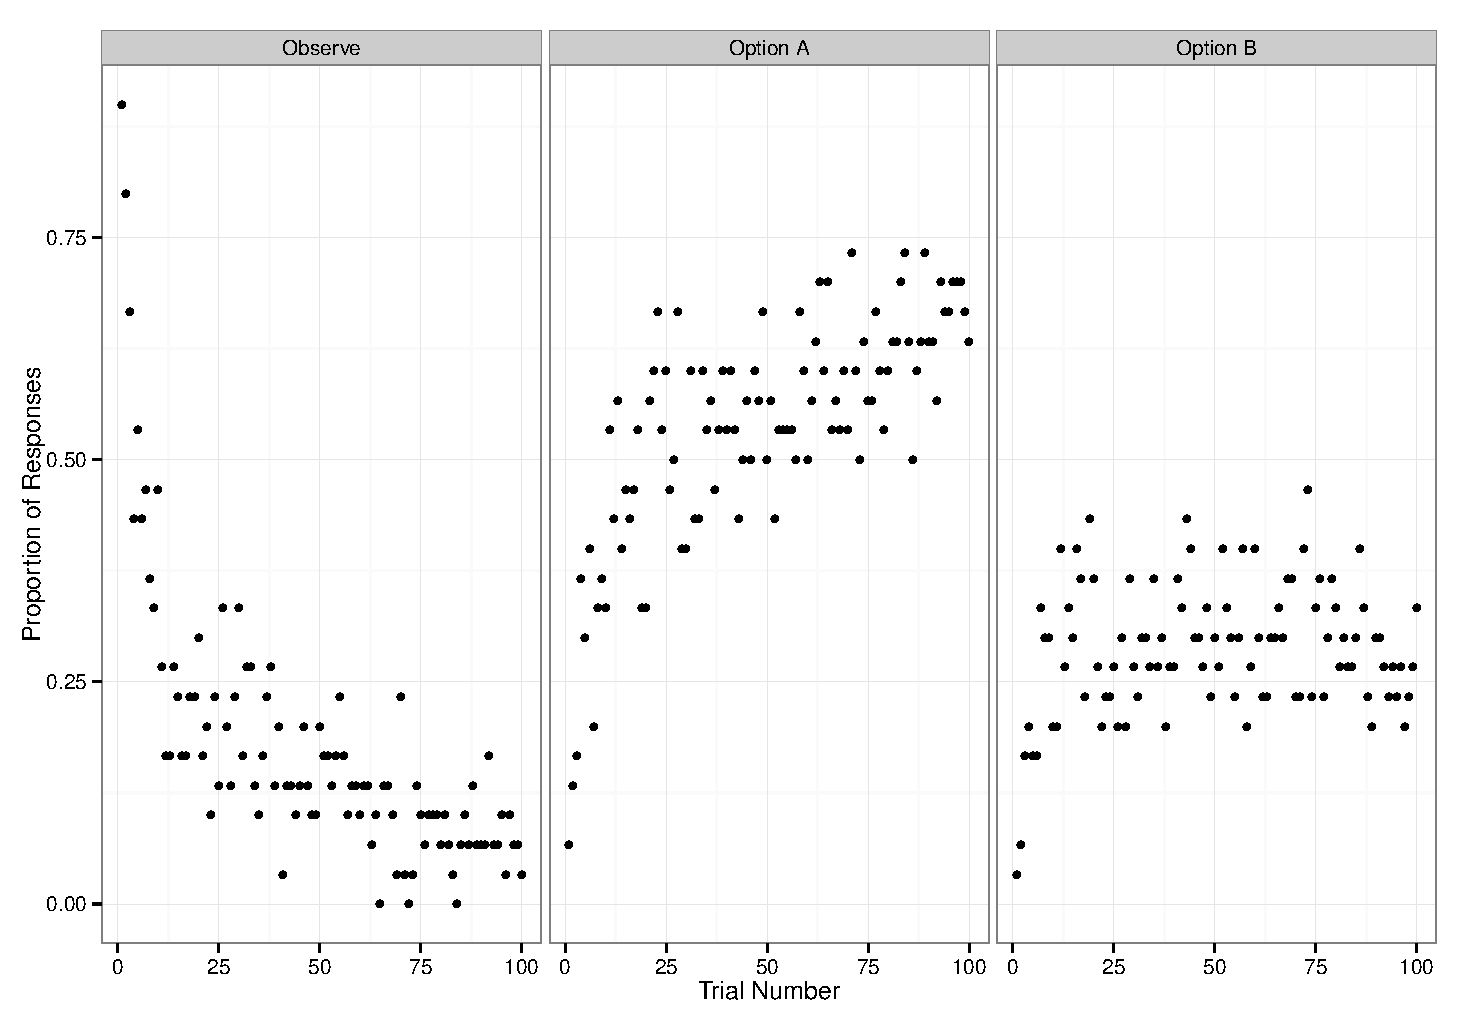
\includegraphics[scale=.5]{realLifeChoices.pdf}
\caption{Response proportions for Experiment 2. The left panel shows the proportion of participants observing on each trial, the middle plots the proportion betting on the high probability color (Option A), and the right panel plots the proportion betting on the low probability color (Option B).}
\label{fig:realLifeChoices}
\end{center}
\end{figure}

The strongest evidence comes from the post-task questionnaire, the results of which are plotted in Figure~\ref{fig:realLifeChoices2}. Although only 5 of 30 participants (17\%) front loaded all observations in the task, there were 12 participants (40\%) who indicated that the front loading strategy was the one they had followed. This discrepancy presumably reflects the fact that many people front loaded most observations but not all of them. The critical finding is that a much larger proportion of participants agreed that the front loading strategy would have won the most money (22 of 30, or 73\%) and indicated that they would follow such a strategy if given the opportunity to do so next time (23 of 30, or 77\%). To check that these results do not simply reflect chance variation in a small sample, we ran Bayesian tests for the equality of proportions under an assumption of uniform priors over proportions: the Bayes factor of 1871:1 in favor of the alternative model is strong evidence that the difference between the 40\% of people who say they front loaded and 77\% of people who say they would do so next time is not due to chance.

Moreover, of the 12 subjects who said they front loaded their observations during the task, only 1 (8\%) indicated that they would switch to a distributed observation strategy. In contrast, of the 16 subjects who indicated that they had distributed their observations during the task, 12 (75\%) indicated that they would switch strategies. Again, we apply a Bayesian test for equality of proportions, and obtain odds of 22467:1 in favour of the hypothesis that people were more willing to switch from distributed observations to a front loading strategy than vice versa.


\begin{figure}[t]
\begin{center}
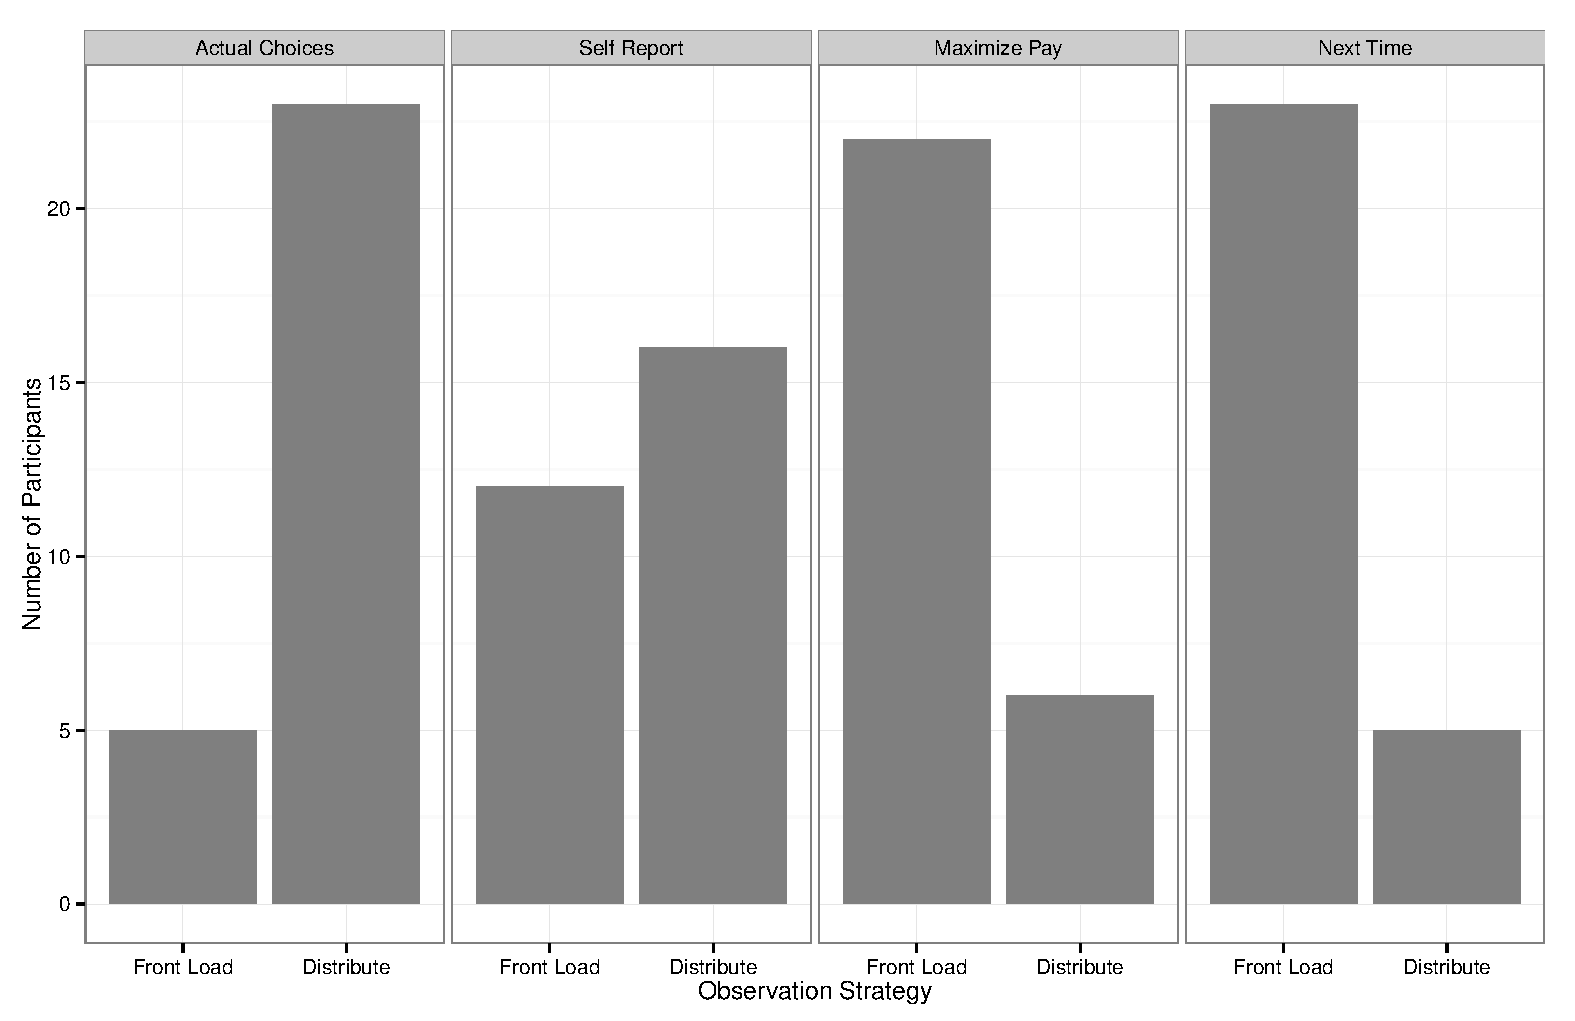
\includegraphics[scale=.5]{RLstrategy.pdf}
\caption{Actual and reported strategies for how observations should be distributed, along with participants' judgments as to which strategy maximizes profits and which would be followed next time. Not shown is the one participant who responded with a ``no observation'' strategy to all questions.}
\label{fig:realLifeChoices2}
\end{center}
\end{figure}

\subsectionX{Discussion}

In Experiment 2, where we provided people with very obvious evidence that the outcome sequences were not rigged in any way, we found no substantial deviations from the strategies that people adopted in Experiment 1. On the other hand, in the post experimental questionnaire, we found very strong evidence that those participants who had not initially followed the optimal strategy {\it were} able to recognize that they had not done so, and correctly identified what strategy they should follow next time. This is entirely consistent with the fact that in Experiment 1, where participants were allowed to play repeated games, this is exactly the shift that happened. Taken together, the results suggest that the need for trial by trial experience, rather than distrust, is the correct explanation. People do not necessarily infer the right strategy purely on the basis of a verbal description: they require direct experience of the task in order to do so \citep[cf][]{newell_role_2007,newell_probability_2013}.

\sectionX{Four Process Models for the Observe or Bet Task}

At the start of the paper we presented the MDP analysis as a rational analysis of the observe or bet task, and used it to motivate testable predictions about how people's behavior should differ in the static and dynamic versions of the problem. Inspired by the MDP model we now introduce a simple approximation to the rational model that can be used to investigate human performance on the observe or bet task in more detail. The model is fairly straightfoward, and consists of a simple evidence accrual rule and a simple but noisy decision rule.

\subsectionX{Evidence Accrual Rules}

The learner maintains an evidence tally that starts at zero. Every time an outcome is observed the tally either increases or decreases by 1. Formally, we let $x_t = 1$ if the learner observes outcome A on trial $t$, $x_t = -1$ if the learner observes outcome B, and $x_t = 0$ if nothing is observed because the learner chose to bet on trial $t$. In the simplest version of the model, the total amount of evidence available at the end of trial $t$ is given by the simple rule:
\begin{equation}
e_t = x_t + e_{t-1}
\label{eq:evidence1}
\end{equation}
In essence, the evidence tally after $t$ trials is simply the number of observed A outcomes minus the number of observed B outcomes. However, there are good reasons to think that people might weight  recent observations more heavily than older ones. The most obvious reason is that, in the dynamic condition in particular, people might have reason to believe that the world has changed and old observations are no longer relevant. Alternatively, people might simply fail to remember older observations. Consistent with the ``constant probability of change'' dynamic model used in our MDP analysis, we propose a simple heuristic in which older evidence decays exponentially, losing some proportion $\alpha$ of its evidentiary value on each trial:\footnote{The parameter in this model is denoted $\alpha$ by analogy with the corresponding parameter in the MDP analysis: since both produce an exponental decay in evidentiary value, it seemed sensible to label them identically. It is worth noting, however, that the MDP model explicitly asserts that this decay is caused by the learner's beliefs about the changeability of the environment, whereas the process model is more agnostic about why the decay occurs. However, as it will turn out, the estimates of the $\alpha$ parameter obtained by fitting the process model support the assumption made by the MDP model.}
\begin{equation}
e_t = x_t + (1-\alpha) e_{t-1}
\end{equation}
Because $\alpha$ governs the rate at which the evidentiary value of observations diminishes over time we refer to it as the {\it evidence decay} parameter. When $\alpha=0$ there is no evidence decay and the evidence accumulation process is equivalent to Equation~\ref{eq:evidence1}. At the other extreme when $\alpha=1$ all older evidence is completely discarded, and the learner relies solely on the most recent event.

\subsectionX{Noisy Responses}

What action does the learner take on trial $t$ given that they have evidence $e_t$? According to the fully optimal MDP analysis, participants should follow the decision strategy outlined in Figure~\ref{fig:behavior}. That is, the learner has a ``decision threshold'' $d_t$ that determines when to observe and when to bet. If the evidence available meets this threshold (i.e., $|e_t| \geq d_t$) then the learner should place a bet, but if it does not (i.e., $|e_t| < d_t$) then they should make another observation. The heuristic model is essentially a noisy version of the same rule. To capture this, we assume normally distributed noise terms $n_t$, where the noise on each trial is generated from a normal distribution with mean 0 and standard deviation $\sigma$. Given these assumptions, the probability that the learner bets on trial $t$ is given by:
\begin{eqnarray}
P(\mbox{bet})
& = & P(|e_t + n_t| \geq d_t)  \nonumber \\
& = & P(e_t + n_t \geq d_t) + P(e_t + n_t \leq -d_t) \nonumber \\
& = & \Phi \left( \frac{e_t - d_t}{\sigma} \right) + \Phi \left( \frac{-e_t - d_t}{\sigma} \right)
\end{eqnarray}
In this expression, $\Phi(\cdot)$ is the cumulative distribution function for a standard normal, and because $\sigma$ governs the amount of noise in the decision process we refer to it as the {\it response stochasticity} parameter.

\subsectionX{Decision Thresholds}

The final ingredient in the model is the form of the decision threshold itself. The simplest version of the model assumes that the decision threshold is a constant value, $d$. Despite its simplicity, this is at odds with the predictions of the MDP model. As Figure~\ref{fig:behavior} illustrates, the rational analysis of the observe or bet task predicts that, at a minimum, the decision threshold $d_t$ is not constant and should decline over time. A simple version of this is instantiated by assuming that the decision thresholds are initially flat, but after some ``critical'' trial they start to decline towards some final value (which may not be zero). We do not claim that this ``piecewise linear'' model is especially realistic, but it captures the key qualitative idea in a fairly simple way.


\subsectionX{Evaluating Four Models of the Task}

The previous discussion suggests four versions of the model. In the full version of the model we allow for the possibility that evidence might decay and allow for declining thresholds using the piecewise linear model. Three alternative models could be produced by removing one or both of these properties. Curiously, all four versions of the model can be viewed as variations on sequential sampling models used in the simple decision making literature \citep{ratcliff_comparison_2004}. For instance, if the evidence tally does not decay and the decision threshold is constant, we obtain a random walk model that is similar in spirit to the highly-successful Weiner diffusion model \citep{ratcliff_theory_1978}. If the decision threshold remains constant and evidence can decay, the resulting model is more closely related to the Ornstein-Uhlenbeck diffusion model and other leaky accumulators \citep{smith_stochastic_2000,usher_time_2001}. In other contexts researchers have argued that when decision deadlines exist the  threshold should decline over time in a fashion similar to the behavior of the MDP model \citep{frazier_sequential_2007}, a topic that has been somewhat contentious in the literature on simple decisions \citep[see, e.g.,][]{shadlen_decision_2013,hawkins_revisiting_2015}

In light of the existing evidence that the ``sequential sampling'' framework can be productively applied as models of strategic ``high level'' decision making tasks \citep{lee_evidence_2004,lee_sequential_2003,lee_decision_2006,newell_right_2011,lee_modeling_2014}, there are good a priori reasons to think that all four models are psychologically plausible. However, only the full model captures {\it all} of the qualitatively important principles embodied by the MDP analysis. If it is truly the case that people are sensitive to the structure of the observe or bet task, we should find that the full model is necessary to account for our data. On the other hand, if people are simply relying on more general strategies, there is no reason to expect this result.

\begin{figure}[p]
\begin{center}
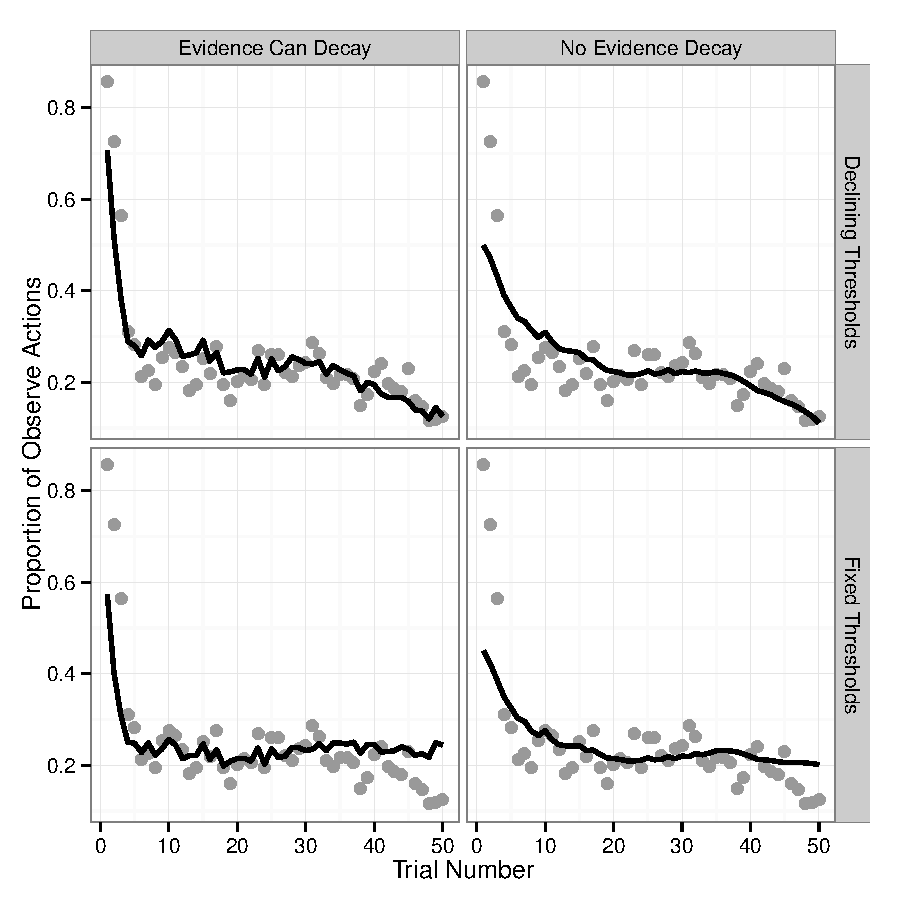
\includegraphics[scale=.5]{modelPredictions2.pdf}
\caption{A visual illustration of why the model requires both the declining thresholds and evidence decay. Grey dots plot the proportion of subjects observing on any given trial for Game 3 in the dynamic condition. The solid lines show the posterior predictive probabilities (i.e., Bayesian model fit) when all four versions of the heuristic model are fit to individual-subject level data.}
\label{fig:modelfits2}
\end{center}
\end{figure}

\begin{table}[p]
\begin{center}
\caption{Quantitative measures of the performance of four different models. The table reports sum squared errors (SSE) for all four models separately for the first 10 trials, the middle 30 trials, and the final 10 trials. A fit is deemed ``adequate'' (and shown in italics) if for a given condition and trial block if it is not more than 50\% worse than the best performing model. The only model that consistently provides adequate fit is the model that allows declining thresholds and evidence decay (shown in bold).}
\label{tab:sse}
\vspace*{6pt}
\footnotesize
\begin{tabular}{r|rr|rrr}
& \multicolumn{2}{|c|}{Model Specification} & \multicolumn{3}{|c}{Model Fit (SSE)} \\
Condition & Declining Threshold & Evidence Decay & Trials 1-10 & Trials 11-40 & Trials 41-50 \\ \hline
\textbf{Static} &  \textbf{Yes} & \textbf{Yes} & \textbf{\textit{0.234}} & \textbf{\textit{0.076}}  & \textbf{\textit{0.004}} \\
Static &  No  & Yes & 0.510          & \textit{0.055}  & 0.084 \\
Static &  Yes & No  & \textit{0.246} & 0.083  & 0.008 \\
Static &  No  & No  & 0.441          & \textit{0.076}  & 0.019 \\ \hline
\textbf{Dynamic} & \textbf{Yes} & \textbf{Yes} & \textbf{\textit{0.689}} & \textbf{\textit{0.160}}  & \textbf{\textit{0.032}} \\
Dynamic & No  & Yes & 1.391          & \textit{0.117}  & 0.276 \\
Dynamic & Yes & No  & 1.209          & 0.207           & \textit{0.036} \\
Dynamic & No  & No  & 1.685          & 0.183           & 0.202
\end{tabular}
\end{center}
\end{table}

We implemented all four models as hierarchical Bayesian models in JAGS, and estimated model parameters using the data from Experiment 1 (see Appendix for details). As it turns out, the full model provides a good fit to the data but the other three models all show theoretically-significant qualitative failures. To illustrate the basic problem, Figure~\ref{fig:modelfits2} plots the posterior predictive values (i.e., model fit) for the observation probabilities in Game 3 of the dynamic condition.\footnote{We note in passing that this procedure is slightly imperfect, and that a Bayes factor analysis would better quantify the strength of evidence for the four models. However, as the results show, the differences in performance between the models are very striking and in the interests of simplicity we forgo introducing this additional complexity.} Each panel corresponds to one of the four models. When the model is allowed to incorporate declining thresholds (top row) it is able to capture the way in which the observation rate falls off over the last 10 trials of the experiment, whereas models with fixed thresholds (bottom row) cannot do so. When the model does not allow for evidence decay (right panels) it cannot simultaneously capture the very high observation rates in the first few trials and the moderate observation rate through the middle of the experiment. When evidence decay is allowed (left panels) it can do so. Notwithstanding the fact that the full model is necessarily the most complex of the four, there is clear evidence that this complexity is necessary. The three other models all show failures to capture theoretically important trends in the data. This intuition is quantified in Table~\ref{tab:sse}, which reports model fits separately for the early trials (1-10), middle trials (11-40) and end trials (41-50). Consistent with the predictions of the MDP analysis, the only process model that consistently provides acceptable fits to the observation profiles at every stage of the task is one that allows for evidentiary decay and declining thresholds.


\subsectionX{Model Performance at the Aggregate and Individual Subject Level}

Before discussing the parameter estimates that emerge from the full model, it is useful to get a sense of how well the full model works.  To that end, Figure~\ref{fig:modelfits1} plots the model fits for all five games in both conditions of Experiment 1.\footnote{Although these plots are aggregated across the three versions of the task, we also confirmed that the model fits were good for each individual version. Similarly, although we estimated parameters separately across all games, versions and conditions, we did verify that parameter estimates tended to be stable within participant, as noted in the Appendix.} As these plots make clear, the model fits at an aggregate level are in very close agreement with the empirical data. There is a slight tendency for the model to underestimate the amount of observation that takes place on the first two trials in the dynamic condition, but this is the only systematic failure.

\begin{figure}[t]
\begin{center}
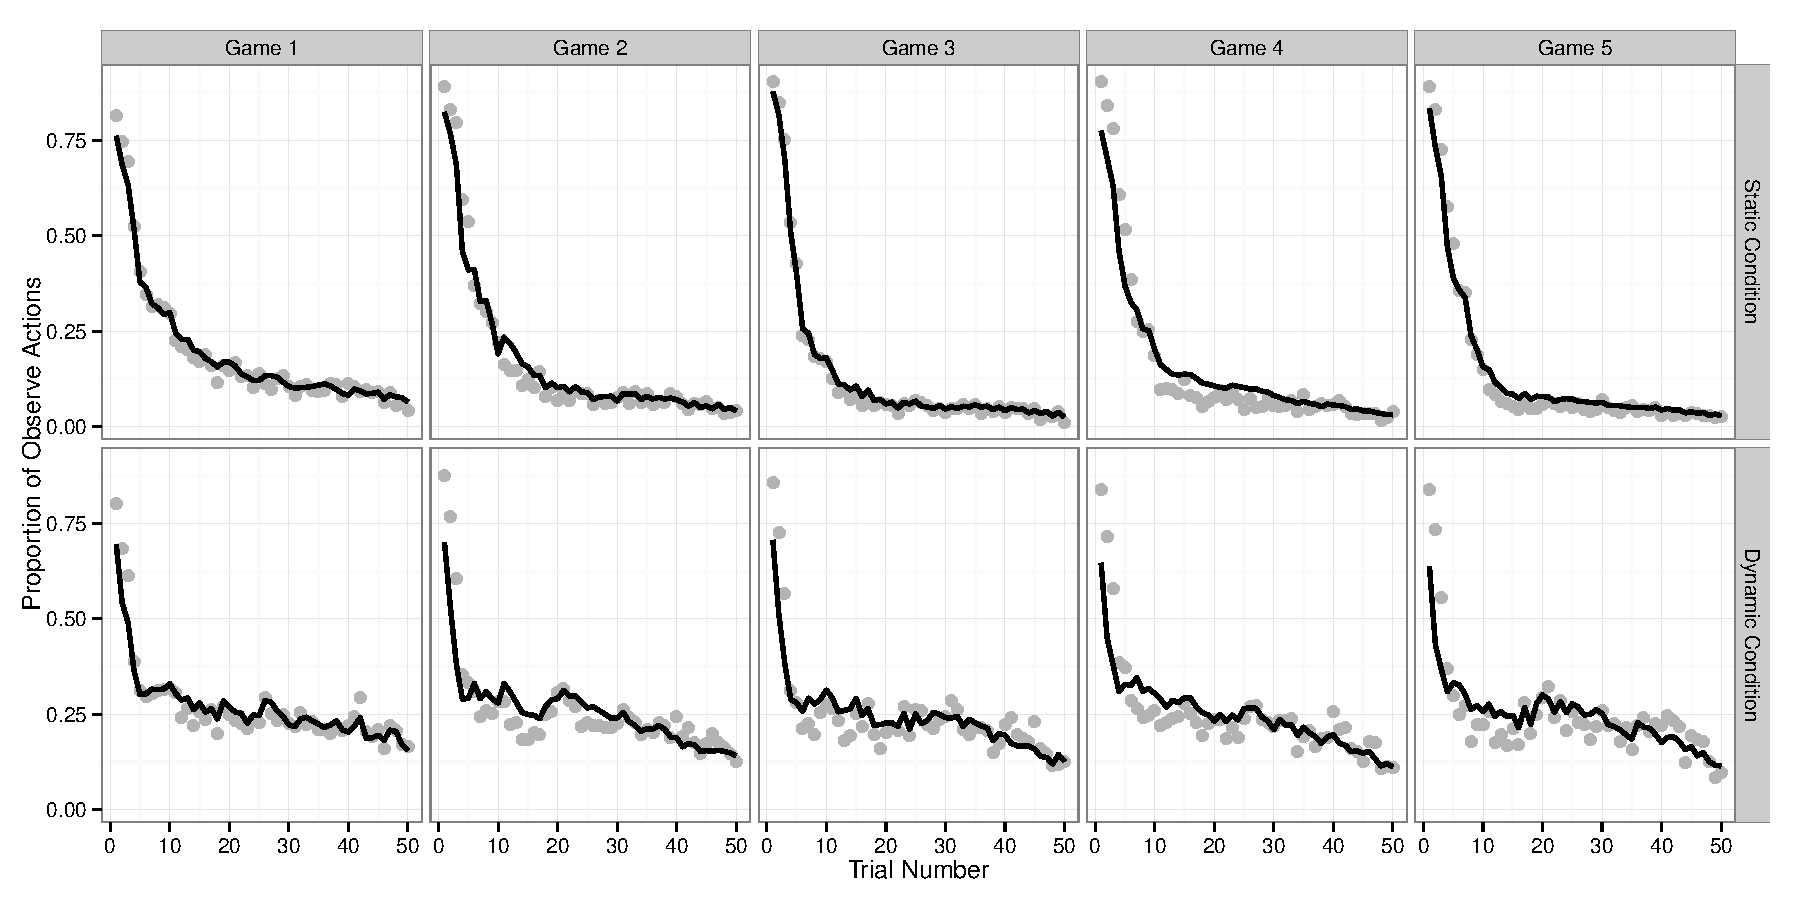
\includegraphics[scale=.5]{modelPredictions1.pdf}
\caption{Observation probabilities estimated when the full version of heuristic model (black lines) is fit to the data from Experiment 1 (grey dots). The model is fit at an individual subject level (see Appendix) and the curves reported here are aggregated across individuals.}
\label{fig:modelfits1}
\end{center}
\end{figure}

%\begin{figure}[p]
%\begin{center}
%\includegraphics[scale=.5]{modellingSpecialCases.pdf}
%\caption{Model fits for the full version of the heuristic model when restricted to the special cases when the static condition and dynamic condition used the same stimulus sequence.}
%\label{fig:modelfits1special}
%\end{center}
%\end{figure}

Moving beyond comparisons at the aggregate level, our approach allows us to go further and examine how well the model captures the behavior of individual subjects. Specifically, we can use the estimated model parameters to construct an ``evidence accumulation plot'' similar to Figure~\ref{fig:behavior} for every participant and every game. The Bayesian data analysis allows us to reconstruct a best estimate of the decision threshold $d_t$ for each person, as well as estimates of the evidence decay parameter $\alpha$ and the response stochasticity $\sigma$. When combined with the empirical data we can estimate the subjective evidence $e_t$ available to each person on every trial. Not every participant is captured well by the model, but given the nature of the data (i.e., each game is just a binary sequence of 50 observe/bet choices) a remarkably large number of them are.

To illustrate the general patterns of variability that the model identifies, eight examples of these estimates are plotted in Figure~\ref{fig:indChoice}.\footnote{Although the decision thresholds used in the model are piecewise linear, what we have plotted in Figure~\protect\ref{fig:indChoice} is the posterior predictive value of the decision threshold $d_t$ at every trial. Because this averages across many different piecewise linear functions, the result can be a smoothed curve, though in most cases the result actually ends up looking fairly similar to a linearly decreasing threshold.} As this plot illustrates there are a range of individual subject strategies that are captured by the model. For instance, panels (a), (b), (c) and (e) all show a participant engaging in a pure ``front loading'' strategy. Participants (a), (b) and (c) all show variations on this strategy: differences in decision threshold $d_t$ produce differences in the number of trials for which the particpant observes (4, 8 and 15, respectively) before switching to a betting-only phase. Because these participants never switch back to observations, the model estimates very small values of $\alpha$ and $\sigma$. Moreover, although this strategy was widespread in the static condition, there are some examples of it (e.g., panel (e)) that appeared -- somewhat inappropriately -- in the dynamic condition.



\begin{figure}[p]
\begin{center}
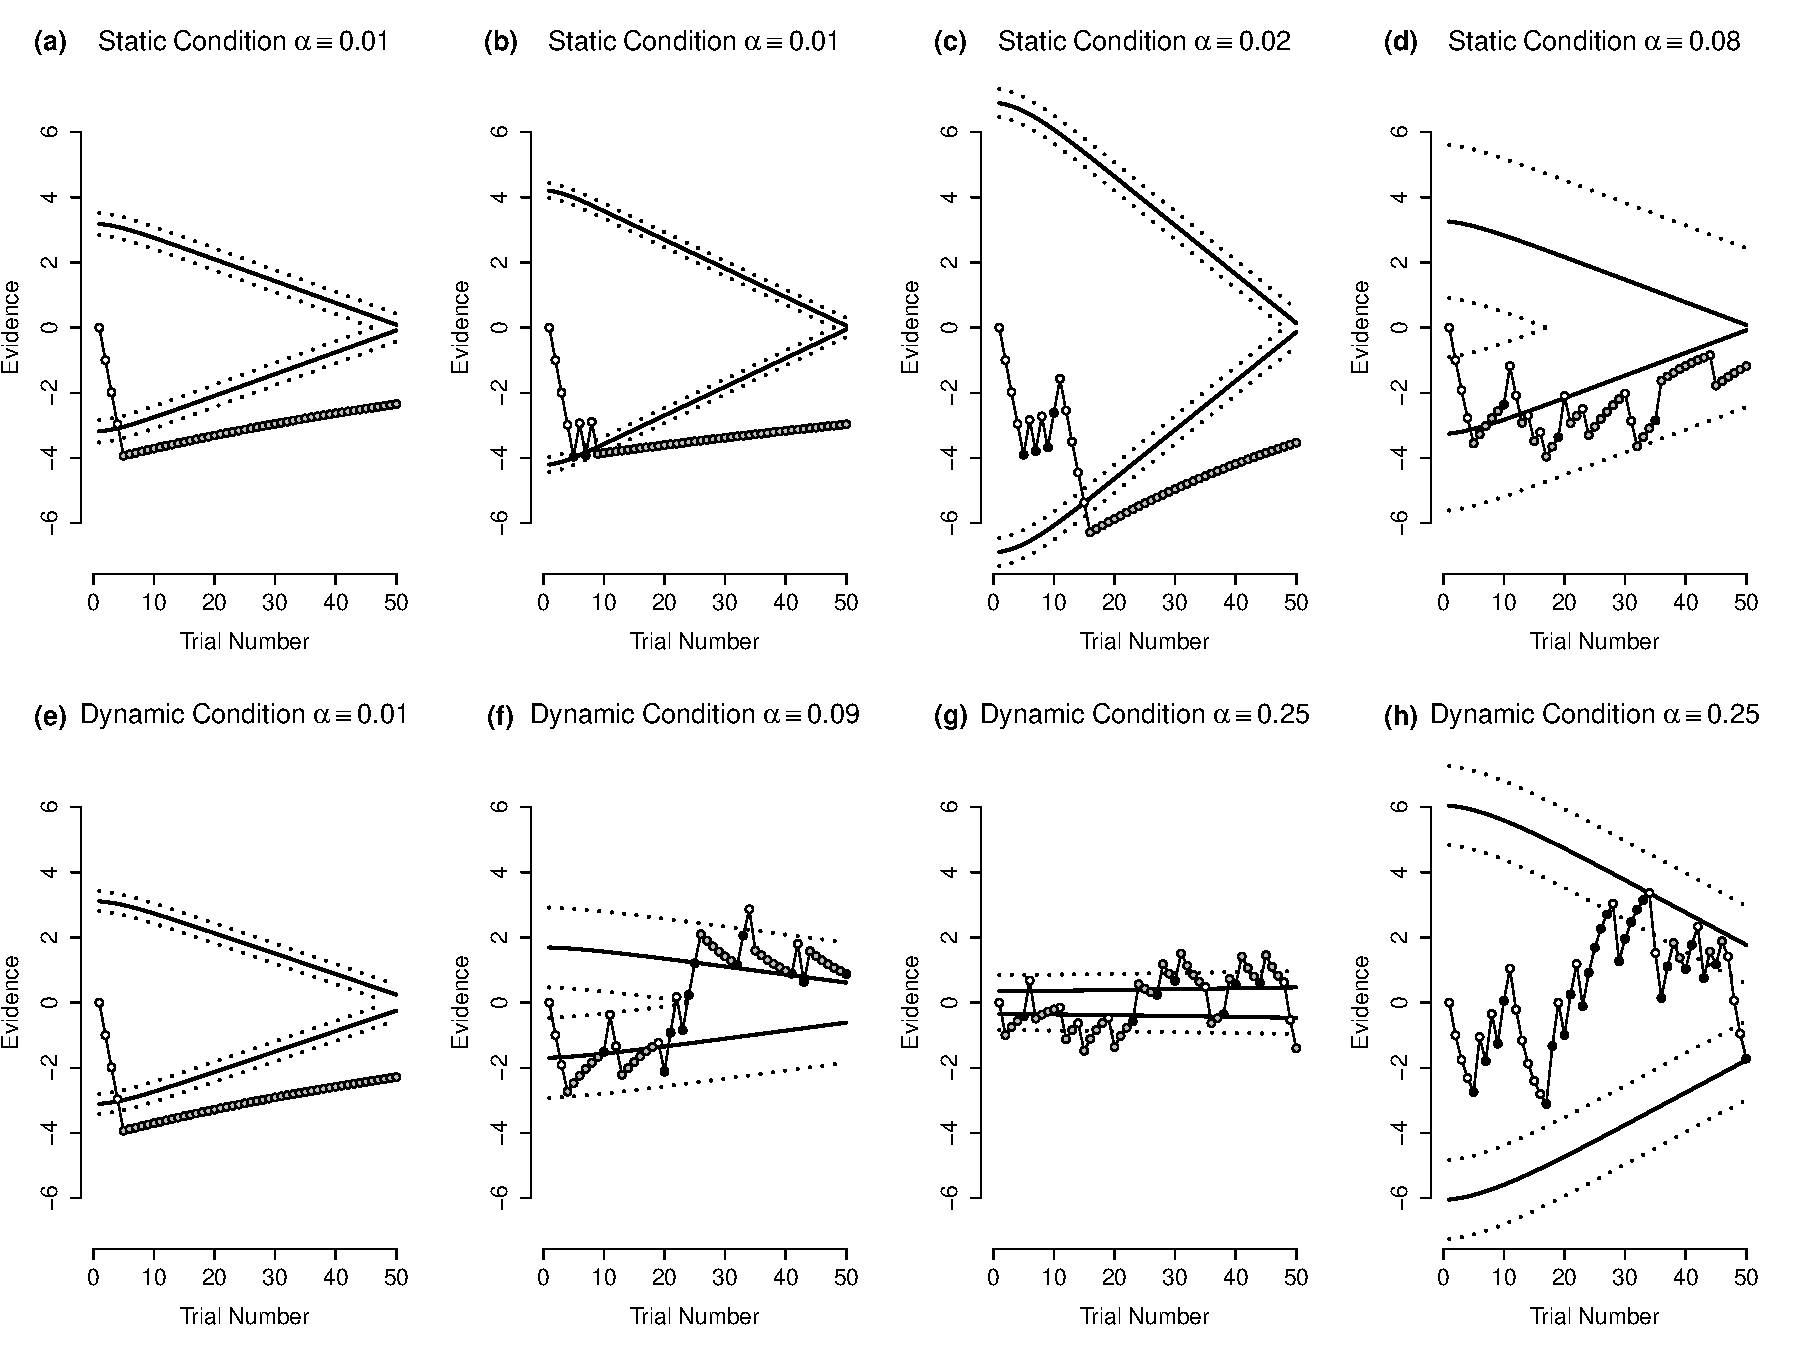
\includegraphics[scale=.5]{indChoice.pdf}
\caption{Reconstructions of individual subject strategies. Each plot depicts the strategy of a single participant in Game 2 Version 1. In each plot, the solid black lines plot the decision threshold $d_t$. However, because responses are assumed to be noisy, the decision threshold is ``soft'': the black line plots the point at which people are equally likely to bet as to observe. To represent the amount of noise, the dotted lines plot one standard deviation $\sigma$ above and below the decision threshold. Black circles denote trials where the participant observed an A outcome, white circles denote trials where they observed a B outcome, and grey circles indicate a bet. Note that in the dynamic condition the change event occurred on trial 17.}
\label{fig:indChoice}
\end{center}
\end{figure}


Many participants adopted a strategy that involved frequent switching between betting and observation, as illustrated in panels (d), (f), (g) and (h). As noted earlier, this was far more common in the dynamic condition than in the static condition. Because it is somewhat difficult to predict precisely when people make these switches, the values of $\sigma$ do tend to be larger in this case, as illustrated by the wider bands plotted in dotted lines. However, it is also notable that the model does tend to extract meaningful patterns from the switches. For instance, consider the participants plotted in panels (d) and (f). Although the participant in panel (f) makes more observations (20 to 15), this is almost entirely due to the fact that panel (f) shows data from the dynamic condition, and the additional observations occur around trial 20-25 shortly after the change point that occurred on trial 17. As the plot makes clear, at this point the participant made a sequence of 6 consective observations that allowed them to detect the change and pushed the evidence tally from below the lower threshold to above the upper threshold. In contrast, the behavior shown in panel (d) comes from the static condition: although the participant periodically made some observations, the evidence tally tended to remain below the lower threshold throughout the entire task.

A final comparison worth noting is between the data sets shown in panel (g) and panel (h). In both cases the model estimates a very high evidentiary decay parameter ($\alpha = .25$), but the decision thresholds are very different in both cases. In panel (g), the participant has very low thresholds, and so what we see is that this person makes one observation followed by a short betting run, followed by another observation and a short betting run, and so on. There is only one occasion where this person made consecutive observations. In contrast, the very high thresholds used by the participant in panel (h) leads them to make 37 consecutive observations at the start of the task, followed by an alternating cycle of bets and observations across the last few trials.


\subsectionX{Parameter Estimates}

\begin{figure}[p]
\begin{center}
\begin{tabular}{ccc}
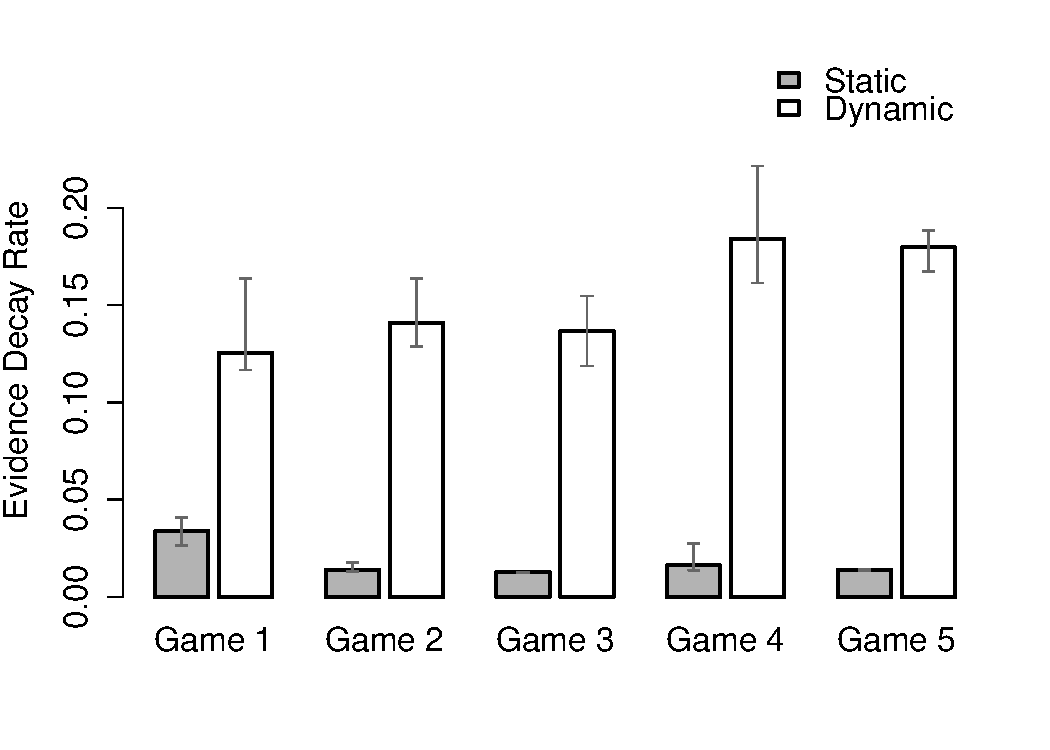
\includegraphics[scale=.4]{decayRate.pdf} & \hspace*{.5cm} &
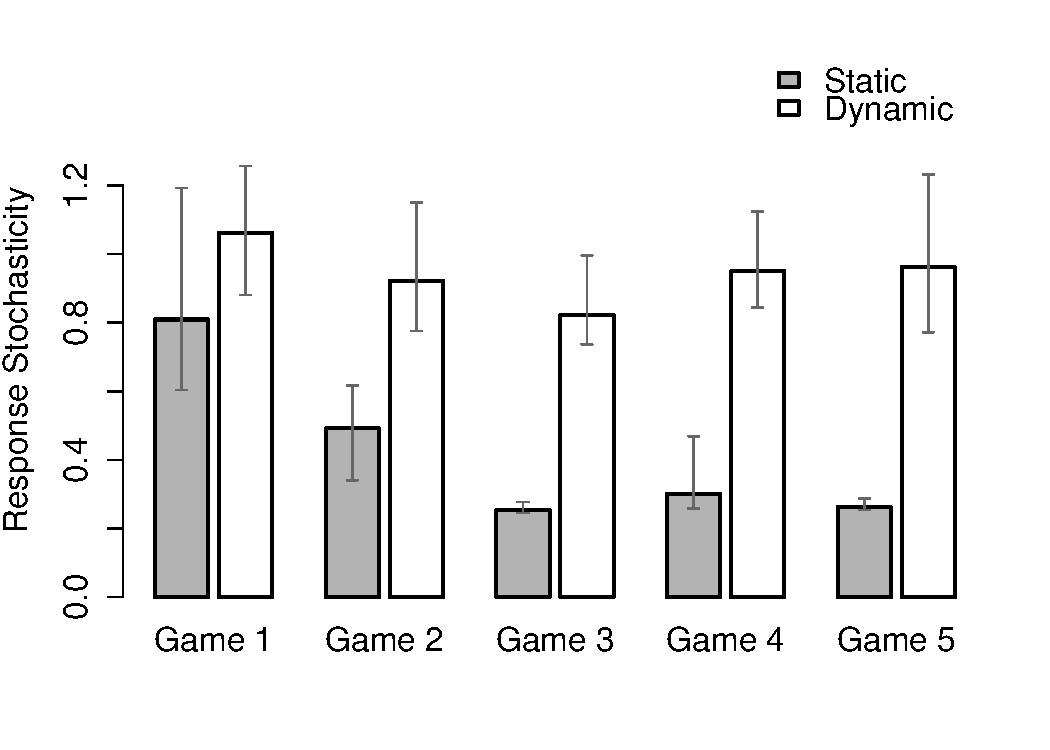
\includegraphics[scale=.4]{responseNoise.pdf} \\
(a) && (b)
\end{tabular}
\caption{Median estimated values of the evidence decay parameter $\alpha$ (panel a) and the response stochasticity parameter $\sigma$ (panel b) as a function of the game and condition, averaged across all three versions of the task and across all participants. Error bars depict 95\% credible intervals constructed using the Bayesian bootstrap \citep{rubin_bayesian_1981}.}
\label{fig:modelpars}
\end{center}
\end{figure}


\begin{figure}[p]
\begin{center}
\includegraphics[scale=.4]{inferredthresholds.pdf}
\caption{Evidence thresholds inferred for participants in Experiment 1. Plots are averaged across participants and across all three versions of the task. Consistent with the predictions made using the MDP model, the evidence thresholds are consistently higher in the static condition than in the dynamic condition, especially early in the task.}
\label{fig:inferredthresholds}
\end{center}
\end{figure}


An interesting picture emerges when we look at the distribution of parameter estimates. For instance, although the heuristic model incorporates the idea that the evidentiary value of observations can decay over time, it is agnostic as to the reason why this occurs. According to the MDP model, the evidentiary value decays because the learner believes that the world might have changed, and as such it makes the strong prediction that the evidence decay rate $\alpha$ should be high in the dynamic condition and very low in the static condition. As Figure~\ref{fig:modelpars}a shows, this is precisely what happens. Not only that, there is a modest learning effect: in the static condition the median value of $\alpha$ is 0.034 on Game 1, which then declines to 0.014 on Game 2 and stays roughly constant for the remainder of the experiment. In the dynamic condition, on the other hand, median $\alpha$ for Game 1 is 0.125, and rises gradually across games until it reaches a value of 0.180 by Game 5.

It is worth noting that this pattern is not an artifact of people's responses becoming less variable across games in the static condition and more variable in the dynamic condition. Indeed, as Figure~\ref{fig:modelpars}b illustrates, the response stochasticity parameter $\sigma$ shows a somewhat different pattern. Although it does show a decline across games in the static condition, it does not show any substantial trend across games in the dynamic condition.

Another respect in which people's performance mirrors the qualitative predictions of the MDP model emerges when we look at the estimated thresholds (averaged across participants) for each game and condition. In Figure~\ref{fig:behavior} we saw that the optimal MDP policy predicts that the decision thresholds should be lower in the dynamic condition than in the static condition. As Figure~\ref{fig:inferredthresholds} illustrates, this is exactly what we find. For all five games, the thresholds in the static condition start out much higher than their counterparts in the dynamic condition, but decline much faster so that by the final trial they are very similar.


\sectionX{General Discussion}

Making good decisions in everyday life requires people to make an exploration-exploitation trade-off. On the one hand, we cannot make good choices if we do not explore our environment  to learn its structure. On the other hand, we cannot gain rewards if we do not exploit our knowledge of this structure to guide our actions and make rewarding choices. The observe or bet task introduced by \citet{tversky_information_1966} represents a very clean experimental tool for investigating how people solve this problem.

Our MDP analysis of this task motivated novel predictions and novel process models for this particular kind of (under-researched) ``pure'' explore-exploit dilemma in static environments as well as in dynamic ones. The conclusion offered by \citet{tversky_information_1966} -- that participants failed to adopt an appropriate strategy -- is at odds with our overall interpretation, and yet the original paper does in some ways foreshadow our findings. In their work Tversky and Edwards included a condition in which participants were (falsely) told that the outcome probabilities might change, and they noted that people did tend to make more observations as a consequence.  However, as our analysis of the task indicates, there is a lot more subtlety to the task than this rather trivial  result suggests. Optimal behavior in a dynamic environment does not simply involve making more observations in order to monitor a changing world; it also requires the learner to lower their evidence thresholds in order to ``strike while the iron is hot''.  Similarly optimal behavior in short tasks with known time horizons (like the 50 trial observe or bet problems) requires that people be sensitive to the short time horizon for the problem, so evidence thresholds should decline over time. In all these respects, people show a striking qualitative agreement with the MDP model.

As noted in the introduction the specific combination of a task in which exploration and exploitation are cleanly separated \citep[cf.][]{sang_learning_2011} and the use of static and dynamic environments allows for  insights that go beyond existing investigations of standard bandit problems. Our conclusions about the remarkable (qualitative) optimality of participants is based both on the simple data analysis (e.g., Figures~\ref{fig:obsByGame}, \ref{fig:frontload2} and \ref{fig:overMatching}) and from fitting a process model to the aggregate and individual data (e.g., Figures~\ref{fig:modelfits2} and \ref{fig:indChoice}). Both types of analyses point to the same conclusion: although people might not behave in a strictly optimal manner, they show an acute sensitivity to the dynamics of the environment, and they show rapid improvement in selecting the correct action (observe or bet) as they gain experience in the task.

These findings are broadly consistent with more standard tasks in which either exploration and exploitation are conflated (to some degree), or static and dynamic tasks are examined in isolation.  For instance, there is evidence for something akin to the front-loading we observed in an exclusively static bandit task: \citet{zhang_cheap_2013} present evidence suggesting that people tend to engage in more exploratory actions early in a bandit problem, though this conclusion was based on a heuristic that defined ``exploratory'' as ``switching options after a win''.  Similarly, \citet{zhang_forgetful_2013} adopt a modeling approach for bandit problems that incorporates a ``forgetfulness'' parameter that has similarities to our approach to handling evidentiary decay. Relatedly, in dynamic versions of the bandit problem (i.e.,  ``restless'' bandits) there is evidence that people continue to switch between options throughout the task \citep[e.g.,][]{speekenbrink_uncertainty_2014,speekenbrink_uncertainty_2015}, consistent with what we find in the dynamic observe or bet task. Moreover, formal analysis of what people should do in a dynamic variant of the standard bandit problem has found people's behavior consistent with an ideal actor model in some but not all respects: although decision makers update beliefs in an optimally reflexive manner, they fail to utilize these beliefs fully for optimal long-term planning (\citealp{knox_nature_2011}; see also \citealp{gureckis_learning_2009} for a similar conclusion regarding the sub-optimality of long-term strategies).

This overall conclusion that participants can approximate optimal solutions but fall short in various (instructive) ways echoes our own findings. For example, one  systematic violation of the MDP prediction found here was that  in both experiments, people seem to show larger departures on the first observe or bet task they encounter. In the static condition, only a minority of participants realized that front loading observations  was the optimal strategy for the task, consistent with the original results by \citet{tversky_information_1966} and those of \citet{rakow_role_2010}. However, it turns out that this special  case is actually the exception and not the rule. When we explicitly asked people what they had learned from a single observe or bet game (Experiment 2) almost everyone agreed that front loading was the optimal strategy and indicated that this is what they would do in future games. Moreover, when they were given the opportunities to play repeated games (Experiment 1) people did in fact make this shift, even though they were given no explicit prompt to consider alternative strategies. This latter finding resonates with \citet{rakow_role_2010} who found that across six consecutive 100 trial games of the static observe-or-bet task, participants slowly learned to distribute their observations in a closer-to-optimal fashion, and with the work of \citep{sang_learning_2011} who also found that people learned with experience in a related task. Interestingly, the improvement in the Rakow et al.\ study emerged despite withholding accuracy feedback until the completion of all six games. This contrasts with Experiment 1 in which detailed feedback was provided at the end of each game. The relatively modest improvements  in front loading behavior observed by \citet{rakow_role_2010}, in contrast to the clear jump in performance between Game 1 and Game 2 of Experiment 1 highlights the power of combining trial-by-trial experience with feedback in tasks of this kind \citep{newell_role_2007}.

How should we reconcile the fact that people show remarkable similarities to the behavior of an optimal agent, yet also fail to perfectly optimize their strategies? One possibility is that  human decision makers simplify the complexity of the problem and thereby produce approximate solutions. The dynamic programming method that we used to compute optimal MDP solutions does not scale well to large real world problems, which makes it impractical for any real world agent \citep[see, e.g.,][for discussion]{van_rooij_rational_INPRESS}. In contrast, the process models used later in the paper are comparatively simple, and in that sense are much more cognitively plausible. However, the heuristic models are very task specific: while the MDP approach can be generalized to other decision making tasks such as bandit problems, the same cannot be said for the  process models. There are a number of more general possiblities for generating heuristics from the MDP approach. For instance, machine learning solutions to realistic sequential decision problems tend to rely on methods that  produce approximate solutions rather than exact ones \citep[e.g.,][]{thrun_monte_1999_fixed,pineau_point-based_2003,silver_monte-carlo_2010}.

Many of these approximate planning algorithms bear similarities to methods currently used by psychologists designing approximately rational cognitive models. For instance, particle filtering is a tool often used when approximating Bayesian learners \citep[e.g.,][]{sanborn_rational_2010,brown_detecting_2009}, and can be naturally extended to approximate optimal decision making  \citep{silver_monte-carlo_2010}. These particle based methods are very similar to simple ``mental simulation'' models of sequential and multi-stage decision making \citep[e.g.,][]{hotaling_dft-d:_2012}, and represent  a promising method for connecting the optimal solution to plausible planning algorithms.

A second perspective emerges when we consider that the most salient deviation from the optimal strategy occurs the first time people need to solve the static version of the task. Moreover the form of the departure is quite striking: by default, people adopt a strategy of repeated switching between observation and betting, a strategy that is far better suited to the dynamic task than the static one. One reason why we might expect to  see this kind of systematic departure was hinted at in the introduction:  so many problems in real life involve dynamic environments, and it makes sense that people's default strategies would be better suited to such a world. Relatedly, it appears that mistaking a changing world for a static one in our task is a ``worse'' failure than the reverse, in the sense that the rewards lost by observing too often in the static task turn out to be smaller than those lost by failing to detect changes in the dynamic one \citep[see][for discussion]{navarro_information_2014}. If this asymmetry holds more generally, then a default strategy of acting as if changes are possible makes a good deal of sense.

A final perspective on this issue arises from the fact that the MDP model is itself a simplification. The MDP model relies on several assumptions that are sensible for the particular task we used in our experiments, but do not hold in all circumstances. For instance, the model expects to encounter abrupt changes in outcome probabilities rather than a gradual drift in the reward contingencies, and in the dynamic conditions it knows roughly how often such changes occur. In that sense it is similar in spirit to an ideal observer model that is given all relevant information about the task, but does not provide a completely general solution for how learners should solve explore-exploit problems in all dynamic environments. One the one hand, this does not greatly influence our central point, which is that people's behavior in this class of problems is -- contrary to the conclusions offered by earlier work -- entirely sensible and in broad agreement with the ideal observer for the task. On the other hand, noting these limits also opens up questions about what a normative standard for real world decision making would look like: human decision making needs to be robust across many different dynamic learning problems, and as such one might expect to see some departures between what people do and what the task-specific MDP model predicts.

More generally, these observations highlight the value of studying human behavior in changing environments. The problem, as we see it, is that human cognition is adapted either via evolution or prior learning to operate in changing and responsive worlds. This matters: as noted by many authors \citep[e.g.,][]{jordan_computational_1999}, the structure of the operating environment imposes strong constraints on how an intelligent agent can be built.  This basic idea underpins both the ``fast and frugal heuristics'' literature \citep[e.g.,][]{simon_rational_1956,gigerenzer_homo_2009} as well as the ``rational  analysis'' approach to building cognitive models \citep[e.g.,][]{anderson_adaptive_1990}. From this viewpoint, one might argue that studying human cognition in an unchanging world can be like studying the aerodynamic properties of an octopus: technically possible, because water and air are both fluids, but frustrating and misleading  because it ignores what the organism is designed to do.


\section{Acknowledgements}

The research in this paper was partially supported via ARC grant DP150104206. DJN received salary support from ARC grant FT110100431 and BRN from ARC grant FT110100151. We thank Tim Rakow, Amy Perfors and Nancy Briggs for helpful comments. Preliminary version of the work was presented at the 36th Annual Conference of the Cognitive Science Society.

\section{References}



%%%%%% end substantive stuff %%%%%

% finish
\bibliography{zot3,zothack}
%\bibliographystyle{elsarticle-num-names}
\bibliographystyle{model5-names}

\appendix

\section{MDP analysis of the observe or bet task}

The probabilistic model that underpins the observe or bet task is assumed to work as follows. On trial $t$ the probability with which the blox machine turns on the blue light is denoted $\theta_t$, and this probability evolves according to the rule:
$$
\theta_t =  \left\{ \begin{array}{ll} \theta_{t-1} & \mbox{ with probability } 1-\alpha \\ \theta_{\mbox{new}} & \mbox{ with probability } \alpha \end{array} \right.
$$
were $\alpha$ denotes the probability that a change occurs on any given trial. When a change occurs, the new outcome probability is drawn from a symmetric beta distribution
$$
\theta_{\mbox{new}} \sim \mbox{Beta}(\phi,\phi)
$$
and for the purposes of our analysis we fix $\phi=1$, corresponding to a uniform distribution over possible $\theta$ values.

\subsection{Optimal behavior in the static task}

Consider the simpler case when the world is static (i.e., $\alpha=0$). At any given point in time $t$, the agent has made some number of observations $n$. Let $n_1$ denote the number of times a ``blue'' outcome has been observed, and let $n_2$ denote the number of times a ``red'' outcome has been seen. These observations do not allow the learner to fully identify the state of the world, since the actual probability $\theta$ remains unknown (we can drop the subscript $t$ in this situation because $\theta$ never changes). Instead, what it determines is a {\it belief} state $b_t$. If our agent is a Bayesian reasoner, then the belief state $b_t$ corresponds to the posterior distribution $P(\theta | n_1, n_2)$. Because each observation is an independent Bernoulli trial with rate parameter $\theta$, this belief state is:
$$
b_t := \mbox{Beta}(\phi+n_1, \phi+n_2)
$$
However, while the belief state comprises a complete distribution over possible values of $\theta$, the properties of the beta distribution mean that it is straightforward to compute the expected probability that the next trial will result in a ``blue'' outcome (i.e., expected value of $\theta$)
$$
E[\theta|n_1, n_2]  = \frac{n_1 + \phi}{n_1+n_2+2\phi}
$$

Viewed as a reinforcement learning problem (i.e. a partially observable Markov decision policy, or POMDP), it is now possible to directly specify the expected reward that will be received on trial $t+1$ given that the learner is in belief state $b_t$ on trial $t$ and undertakes action $a$. Define $a=0$ to be the ``observe" action, $a=1$ to be the ``bet blue" action, and $a=2$ to be ``bet red" action. The expected reward $r_{t+1}$ for moving {\it out} of belief state $b_t$ via action $a$ is given by:
$$
r_{t+1}^a = \left\{ \begin{array}{rl} 0 & \mbox{ if } a=0 \\ \\ \frac{n_1 + \phi}{n_1+n_2+2\phi} & \mbox{ if } a=1 \\ \\ \frac{n_2 + \phi}{n_1+n_2+2\phi} & \mbox{ if } a=2 \end{array} \right.
$$
Similarly, it is straightforward to define the transition probabilities that describe how the belief state will change as a function of the actions that the agent makes. If the agent bets (i.e., $a=1$ or $a=2$), then no observations are made available, so the belief state does not change (i.e., $b_{t+1} = b_t$ with probability 1). On the other hand, if the agent observed (i.e., $a=0$) then
$$
b_{t+1} = \left\{
\begin{array}{rl}
\mbox{Beta}(\phi + n_1 + 1, \phi + n_2 ) & \mbox{ with probability } \frac{n_1 + \phi}{n_1+n_2+2\phi} \\ \mbox{Beta}(\phi + n_1, \phi + n_2 + 1 ) & \mbox{ with probability } \frac{n_2 + \phi}{n_1+n_2+2\phi}
\end{array}
\right.
$$
This defines a very simple POMDP for which we can infer the optimal policy using value iteration. Because the relationship between observations and beliefs is so simple, the size of the set of actually-reachable beliefs is the same as the size of the set of observation states (i.e., possible values for $n_1$ and $n_2$) so we don't need to do anything complicated. The utility of any given belief state $b_t$ on trial $t$ is given by Bellman's equation. The only subtle thing to note is that, because rewards in the observe or bet task are given contingent on the {\it previous} action, the ``immediate'' reward for state $b_t$ is in fact determined by $r_{t+1}^a$, the reward for moving into the next trial after taking action $a$. (One simply has to remember that even the final trial of the experiment generates a reward, even though no follow up action is possible). When written this way, the utilities must satisfy:
$$
u(b_{t}) =  \max_{a} \left( r_{t+1}^a + \sum_{a} u(b_{t+1}) P(b_{t+1} | b_t, a) \right)
$$
This is a slightly unusual way to write Bellman's equations, because the usual specification of the MDP problem assumes that the reward generated by any state is independent of the action that brought you into it, and this does not hold for the observe or bet task. The optimal policy shown in Figure~\ref{fig:behavior}a is computed using this specification of the problem. Strictly speaking, the decision policy is defined with respect to the two counts, $n_1$ and $n_2$ as well as the trial number $t$, but it turns out that the {\it difference} $n_1 - n_2$ and the trial number $t$ are very nearly a sufficient statistic for determining the action, and for this reason the decision policies discussed in the main text define the policy in those terms.

\subsection{Optimal behavior in the dynamic task}

Computing optimal policies for dynamic environments is more difficult. A slightly simplified way of computing decision policies in the dynamic version of the task is outlined below. Suppose the learner believes that on every trial there is some probability that the outcome probability $\theta$ is redrawn, as per the generative model discussed at the beginning. That is, what happens if the agent sets $\alpha > 0$? Again, let's start with a slightly simpler case than the full problem facing the human participants. Suppose that the change points were actually announced to participants when they occurred. What this would mean is that the learner knows the true values for $n_1$ and $n_2$, where $n_1$ and $n_2$ now refer to the number of observed ``blue" and ``red" outcomes {\it since the most recent change}. Under these conditions, the POMDP analysis proceeds exactly as before, except that the transition rule for the belief states when an observe action ($a=0$) is made now becomes:
$$
b_{t+1} = \left\{
\begin{array}{rl}
\mbox{Beta}(\phi + n_1 + 1, \phi + n_2 ) & \mbox{ with probability } (1-\alpha) \frac{n_1 + \phi}{n_1+n_2+2\phi} \\ \mbox{Beta}(\phi + n_1, \phi + n_2 + 1 ) & \mbox{ with probability } (1-\alpha) \frac{n_2 + \phi}{n_1+n_2+2\phi} \\
\mbox{Beta}(\phi, \phi ) & \mbox{ with probability } \alpha
\end{array}
\right.
$$
and when a bet action is made it becomes
$$
b_{t+1} = \left\{
\begin{array}{rl}
\mbox{Beta}(\phi + n_1, \phi + n_2 ) & \mbox{ with probability } (1-\alpha) \\
\mbox{Beta}(\phi, \phi ) & \mbox{ with probability } \alpha
\end{array}
\right.
$$

In other words, the agent knows that on every trial it will be sent back to the beginning state (i.e. zero relevant observations) with probability $\alpha$. This by itself has an effect on the optimal policy. It is this specification of the problem that leads to the policy shown in Figure~\ref{fig:behavior}b

That being said, the actual belief state $b_t$ for a Bayesian learner in the dynamic task is somewhat more complicated than simply counting $n_1$ and $n_2$. Because the actual change point is unobserved, the learner must maintain a full posterior distribution over $n_1$ and $n_2$ given the observations that have been made. This posterior distribution can be efficiently estimated using particle filtering, and we approximate the behavior of the optimal learner by choosing to bet only if the posterior expected value of $n_1 - n_2$ exceeds the relevant threshold.

\section{Data analysis model}


One advantage to the MDP analysis is that it yields a genuine prediction about the experiment, one that is not especially dependent on free parameters. Specifically, it predicts a very distinctive profile for the difference in observation rates between conditions: an initial decline, followed by a sharp rise, followed by a curvilinear pattern. However, on its own the model does not go further than this qualitative prediction. It does not in any meaningful sense specify a complete probabilistic model for human responses on any given trial. One possibility when analyzing empirical data in light of such predictions is to augment the ideal observer model with additional assumptions about response generation \citep[e.g.,][]{navarro_sampling_2012,hemmer_moving_INPRESS} and then use Bayesian methods for our data analysis. Unfortunately, the complexity of the MDP model makes that infeasible in this case because of the difficulty even to extract a prediction from the model. An alternative possibility is to begin with the key {\it qualitative} constraint, and then construct a proper statistical model that embodies exactly that constraint. This idea has considerable merit in its own right: previous authors have argued that cognitive models are typically intended only to specify qualitative predictions \citep{pitt_global_2006}, and if so it makes sense to assess them in such terms. For the observation rates data, the ``decline, then rise, then curve'' prediction corresponds to the following non-linear regression spline model:
$$
d_t = \left\{ \begin{array}{ll}
b_0 + b_1 t & \mbox{ if }  t  \in [0, c_1] \\
b_0 + b_1 c_1 + b_2 (t-c_1) & \mbox{ if }  t \in [c_1, c_2]  \\
b_0 + b_1 c_1 + b_2 (c_2-c_1) + b_3 (t-50)(t-c_2)& \mbox{ if }  t \in [c_2, 50]
\end{array} \right.
$$
An illustration of this regression function is shown in Figure~\ref{fig:spline}. In this plot, the two black dots mark the locations of the change points, $c_1$ and $c_2$, which divide the regression function into three segments. The intercept is denoted $b_0$, the slope of the first segment is $b_1$, the slope of the second segment is $b_2$, and the curvature of the third segment is $b_3$. The general form of the regression function is inspired by the MDP analysis, but we set diffuse priors over the regression parameters. Priors over the $b$ coefficients are normal with mean $\mu=0$ and precision $\tau=10^{-4}$. The prior over the precision $\tau$ of the data is a gamma with shape and scale of $10^{-3}$. Priors over the location of change points are set to be similarly diffuse.

\begin{figure}[t]
\begin{center}
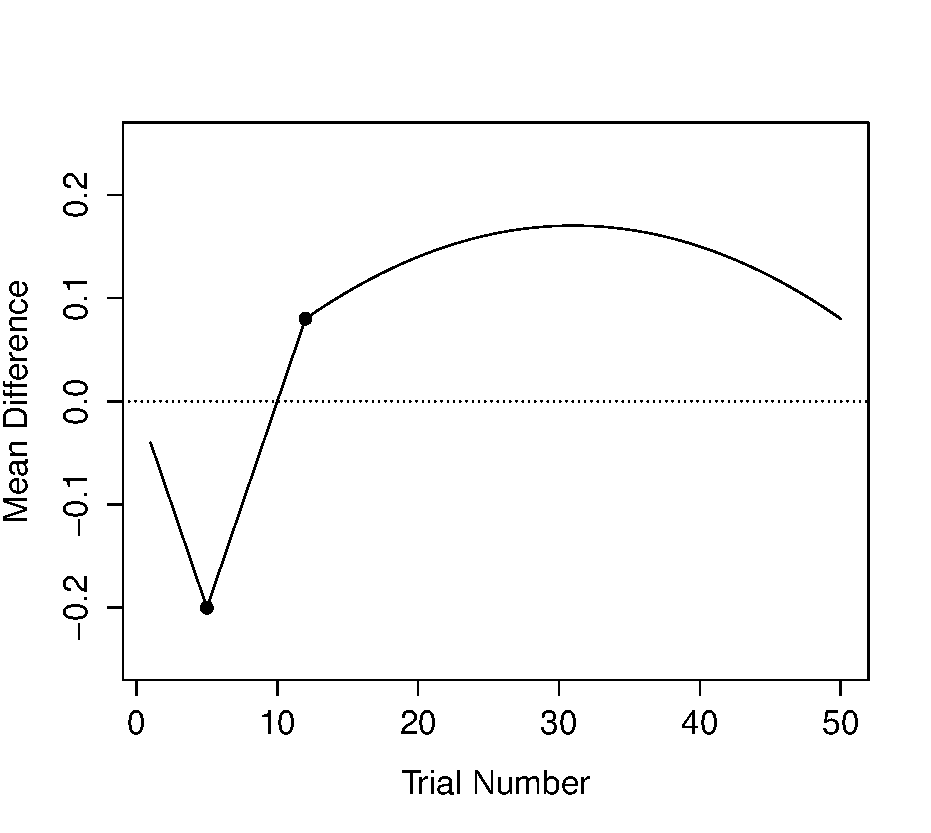
\includegraphics[scale=0.5]{regressionModel.pdf}
\caption{The non-linear regression spline used to analyze the results of Experiment 1.}
\label{fig:spline}
\end{center}
\end{figure}




\section{Additional details regarding the heuristic models}

The main text describes the theoretically important aspects to the heuristic models, but does not describe the priors used in our JAGS implementation of these models. Our approach was as follows. First, we estimated model parameters independently for every distinct stimulus sequence (i.e., all five games, three versions and two conditions). The reason for doing so was partially convenience (the JAGS implementation becomes somewhat complicated otherwise) and partially to avoid placing strong priors over how these different cases should be related to each other. For any one case, however, we used a Bayesian hierarchical model with the following structure. If the response stochasticity parameter for the $i$-th subject is denoted $\sigma_i$, then we can write our hierarchical model as follows:
$$
\begin{array}{rcl}
\sigma_i &\sim& \mbox{Exp}(\lambda) \\
\lambda &\sim& \mbox{Gamma}(1,1)
\end{array}
$$
For the evidence decay parameter $\alpha$, in those models that allowed values other than $\alpha=0$, we adopted the following prior:
$$
\begin{array}{rcl}
\alpha_i &\sim& \mbox{Beta}(a_1+1,a_2+1) \\
a_j &\sim& \mbox{Gamma}(1,1)
\end{array}
$$
Depending on whether the model allowed declining thresholds or not, the decision threshold $\bm{d}_t$ could be described in one of two ways. In both cases, there was an ``initial value'' for the decision threshold $d_{0}$ for which the following hierarchical prior was used:
$$
\begin{array}{rcl}
d_{0i} &\sim& \mbox{Gamma}(g_{01},g_{02}) \\
g_{0j} &\sim& \mbox{Exp}(1)
\end{array}
$$
If the model allowed declining thresholds we also included an ``end value'' for the decision threshold $d_{1}$ that indicated the evidence level required to justify betting on the final trial. The prior over this parameter was specified in the same way as the prior over the initial threshold:
$$
\begin{array}{rcl}
d_{1i} &\sim& \mbox{Gamma}(g_{11},g_{12}) \\
g_{1j} &\sim& \mbox{Exp}(1)
\end{array}
$$
Finally, in order to capture the idea that the threshold stays flat for some number of trials and only then begins to decline, we included a threshold-change parameter $c$ that indicated the proportion of trials over which the initial flat region extends (e.g., if $c=.2$ then the threshold stays flat for the first 20\% of trials; i.e., first 10 trials) and then declines linearly. The prior over $c$ was specified as:
$$
\begin{array}{rcl}
c_i &\sim& \mbox{Beta}(b_1+1,b_2+1) \\
b_j &\sim& \mbox{Gamma}(1,1)
\end{array}
$$
It should be noted that these priors were adopted primarily for convenience. We ran a few additional simulations to check that the model is robust to the choice of prior. Overall, we found that although there is some sensitivity to the precise model specification the theoretically important results are not sensitive to the prior: across many different versions of the prior we found that the full model (i.e., declining thresholds plus evidence decay) performed best, and that the parameter estimates across different games and conditions always showed the same qualitative pattern as those shown in Figure~\protect\ref{fig:modelpars}. Nevertheless, some degree of caution is warranted in regards to low-level details: it appears to be the case that {\it some} form of declining threshold is necessary to account for the data (as  Figure 12 shows, a fixed threshold does not work), but we suspect that the piecewise linear model that we have used in this paper is likely to be inaccurate.

These caveats notwithstanding, it is noteworthy that the parameter estimates tended to be stable across games played by the same participant, suggesting that variability in model parameters does capture stable individual differences in performance. For instance, the average within-subject correlation between the $\alpha$ value between different games was $r=0.67$, computed separately for each pair of games, and for each version and condition in order to avoid conflating the effect of experimental manipulation with the estimate of within-subject correlation. Estimates for the initial value of the threshold $d_1$ were slightly less stable at $r=0.50$, as were the final threshold values $d_{50}$ at $r=0.41$. The least stable parameter was the response noise $\sigma$, at $r=0.38$.

\section{List of sequences used in Experiment 1}

In abstract terms, the stimuli in an observe or bet task can be characterized as a binary sequence of outcomes, with 0s corresponding to one outcome and 1s corresponding to the other. The stimulus sequences used in the static condition were as follows:

\begin{center}
\begin{tabular}{l|l}
Version 1, Game 1 & \texttt{00000100001000000100000011000000010000001001011000}\\
Version 1, Game 2 & \texttt{00001010110000000010010000010000011000000100001110}\\
Version 1, Game 3 & \texttt{11111011011111111111100011101111010110001101111011}\\
Version 1, Game 4 & \texttt{00000000000101100010011110000000000000101011000000}\\
Version 1, Game 5 & \texttt{11111111101111101101111110110011101111111110111110}\\ \hline
Version 2, Game 1 & \texttt{00000001100100010110000010000001101000010010010000}\\
Version 2, Game 2 & \texttt{00001010011000000100000000100110010110001000011000}\\
Version 2, Game 3 & \texttt{00000001000001010000000100101010111000000000100100}\\
Version 2, Game 4 & \texttt{01010110101100111110011111111111101110011111111111}\\
Version 2, Game 5 & \texttt{10101111111111111111100111101111110100011111011111}\\ \hline
Version 3, Game 1 & \texttt{01110101011110111111111111111101111011101111101111}\\
Version 3, Game 2 & \texttt{11101111101111111111011111111010111011011110011111}\\
Version 3, Game 3 & \texttt{00000000110110000000000000000010000000001010000000}\\
Version 3, Game 4 & \texttt{11110111111111110111000111111101110110111111111111}\\
Version 3, Game 5 & \texttt{11110010011111101001011011111111110111100111101111}\\
\end{tabular}
\end{center}


\noindent
The stimulus sequences used in the dynamic condition were as follows. Trials listed in italics correspond to events that occurred after the change point:


\begin{center}
\begin{tabular}{l|l}
Version 1, Game 1 & \texttt{00000100001000000100000011000000010000001001011000}\\
Version 1, Game 2 & \texttt{00001010110000001\textit{101101111101111100111111011110001}}\\
Version 1, Game 3 & \texttt{11111011011111111111100010\textit{010000101001110010000100}}\\
Version 1, Game 4 & \texttt{00000000000101100010011110001\textit{111111111010100111111}}\\
Version 1, Game 5 & \texttt{1111111110111110110110\textit{0001001100010000000001000001}}\\ \hline
Version 2, Game 1 & \texttt{00000001100100010110000010000001100\textit{111101101101111}}\\
Version 2, Game 2 & \texttt{0000101001100001\textit{1011111111011001101001110111100111}}\\
Version 2, Game 3 & \texttt{00000001000001010000000100101010111000000000100100}\\
Version 2, Game 4 & \texttt{01010110101100111111\textit{100000000000010001100000000000}}\\
Version 2, Game 5 & \texttt{101011111111111110\textit{00011000010000001011100000100000}}\\ \hline
Version 3, Game 1 & \texttt{01110101011110111111110\textit{000000010000100010000010000}}\\
Version 3, Game 2 & \texttt{11101111101111110\textit{000100000000101000100100001100000}}\\
Version 3, Game 3 & \texttt{0000000011011000001\textit{1111111111101111111110101111111}}\\
Version 3, Game 4 & \texttt{11110111111111110110\textit{111000000010001001000000000000}}\\
Version 3, Game 5 & \texttt{11110010011111101001011011111111110111100111101111}\\
\end{tabular}
\end{center}

\end{document}




